\documentclass[
	12pt,
	openright,
	twoside,
	a4paper,
	english,
	brazil
	]{abntex2}

\usepackage{lmodern}
\usepackage[T1]{fontenc}
\usepackage[utf8]{inputenc}
\usepackage{indentfirst}
\usepackage{color}
\usepackage{float}
\usepackage{graphicx}
\usepackage{microtype}
\usepackage[brazilian,hyperpageref]{backref}
\usepackage[alf]{abntex2cite}
\usepackage{amsmath}
\usepackage{ufsc}
\usepackage{listings}
\usepackage{cleveref}
\usepackage{multirow}
\usepackage{longtable}

\renewcommand{\backrefpagesname}{Citado na(s) página(s):~}
\renewcommand{\backref}{}
\renewcommand*{\backrefalt}[4]{
	\ifcase #1
		Nenhuma citação no texto.
	\or
		Citado na página #2.
	\else
		Citado #1 vezes nas páginas #2.
	\fi}

%------------------------------------------------------------------------------%

\titulo{Dinâmica para análise e identificação de riscos em equipes ágeis}
\autor{Amanda Martins Oliveira}
\local{Florianópolis, Brasil}
\data{2024}
\orientador{Jean Carlo Rossa Hauck}
%\coorientador{}
\instituicao{
  Universidade de Santa Catarina -- UFSC
  \par
  Ciências da Computação
  \par
  Programa de Graduação}
\tipotrabalho{Tese (Bacharel)}
\preambulo{Trabalho de Conclusão de Curso submetido ao curso de Ciências da Computação como requisito para a obtenção do Grau de Bacharel em Ciências da Computação.}

% ABNT ------------------------------------------------------------------------%

\graphicspath{ {./images/} }
\definecolor{blue}{RGB}{41,5,195}

\makeatletter
  \hypersetup{
    pdftitle={\@title},
    pdfauthor={\@author},
    pdfsubject={\imprimirpreambulo},
    pdfcreator={LaTeX with abnTeX2},
    pdfkeywords={abnt}{latex}{abntex}{abntex2}{trabalho acadêmico},
    colorlinks=true,
    linkcolor=blue,
    citecolor=blue,
    filecolor=magenta,
    urlcolor=blue,
    bookmarksdepth=4
  }
\makeatother

\makeatletter
  \setlength{\@fptop}{5pt}
\makeatother

\setlength{\parindent}{1.3cm}
\setlength{\parskip}{0.2cm}

% Other settings --------------------------------------------------------------%

\crefformat{footnote}{#2\footnotemark[#1]#3}
\lstset{
  basicstyle=\small\ttfamily,
  columns=flexible,
  breaklines=true,
  literate=
    {á}{{\'a}}1
    {à}{{\`a}}1
    {ã}{{\~a}}1
    {é}{{\'e}}1
    {ê}{{\^e}}1
    {í}{{\'i}}1
    {ó}{{\'o}}1
    {õ}{{\~o}}1
    {ú}{{\'u}}1
    {ü}{{\"u}}1
    {ç}{{\c{c}}}1
}

%------------------------------------------------------------------------------%

\makeindex

%------------------------------------------------------------------------------%

\begin{document}
\selectlanguage{brazil}
\frenchspacing

%------------------------------------------------------------------------------%

\imprimircapa

%------------------------------------------------------------------------------%

\imprimirfolhaderosto*

%------------------------------------------------------------------------------%

\setlength{\absparsep}{18pt}
\begin{resumo}
  Com a popularização dos métodos ágeis cada vez mais organizações adotam este abordagem pela flexibilidade  e adaptabilidade proposta pelo modelo. Entretanto, apesar destas vantagens o uso destes métodos traz consigo desafios relacionados à gestão de riscos nos projetos, já que frequentemente não possuem um processo explícito para tal gerenciamento.
  O objetivo deste trabalho é analisar, desenvolver, aplicar e avaliar uma dinâmica que auxilie no processo de gestão de riscos, por meio de um estudo de caso aplicado em equipes ágeis e em sala de aula. A proposta é criar uma maneira lúdica e facilitada de gerenciamento de riscos, adaptada para ambientes ágeis.
  Para isto o trabalho será baseado em uma estrutura que inicia com uma fundamentação teórica e a análise do estado da arte sobre a gestão de riscos em metodologias ágeis. Com base nessa análise, será desenvolvida uma dinâmica para gestão de riscos no contexto ágil. Em seguida, a eficácia dessa dinâmica será avaliada por meio da aplicação em estudos de caso com equipes de desenvolvimento de software e em cenários educacionais, como salas de aula.
  Espera-se com isso o desenvolvimento e a validação de uma dinâmica lúdica que auxilie os profissionais que utilizam metodologias ágeis na análise e identificação de riscos. Acredita-se que, com essa abordagem, será possível mitigar impactos negativos potenciais nos projetos, promovendo uma entrega de valor contínua e eficiente pelas equipes que integrarem a ferramenta ao seu processo. 
  \vspace{\onelineskip}

  \noindent\textbf{Palavras-chave}: Gestão de Riscos, Gestão de Projetos, Métodos Ágeis.

\end{resumo}

%------------------------------------------------------------------------------%

\begin{resumo}[Abstract]
  \begin{otherlanguage*}{english}
    With the popularization of agile methods, an increasing number of organizations are adopting this approach due to the flexibility and adaptability proposed by the model. However, despite these advantages, the use of these methods brings challenges related to risk management in projects, as they often lack an explicit process for such management.
    The objective of this study is to analyze, develop, apply, and evaluate a framework that aids the risk management process through a case study applied to agile teams and in classroom settings. The proposal is to create a playful and simplified way of managing risks, adapted for agile environments.
    To achieve this, the work will be based on a structure that begins with a theoretical foundation and an analysis of the state of the art regarding risk management in agile methodologies. Based on this analysis, a risk management framework will be developed for the agile context. Subsequently, the effectiveness of this framework will be evaluated through application in case studies with software development teams and in educational scenarios, such as classrooms.
    The aim is to develop and validate a playful framework that assists professionals using agile methodologies in the analysis and identification of risks. It is believed that this approach will help mitigate potential negative impacts on projects, promoting continuous and efficient value delivery by teams that integrate the tool into their processes.
    \vspace{\onelineskip}

    \noindent\textbf{Keywords}: Risk management, Project Management, Agile Methods.
  \end{otherlanguage*}
\end{resumo}

% Figuras ---------------------------------------------------------------------%

\pdfbookmark[0]{\listfigurename}{lof}
\listoffigures*
\cleardoublepage

% Quadros ---------------------------------------------------------------------%

% \pdfbookmark[0]{\listofquadrosname}{loq}
% \listofquadros*
% \cleardoublepage

% % Tabelas ---------------------------------------------------------------------%

\pdfbookmark[0]{\listtablename}{lot}
\listoftables*
\cleardoublepage

% Siglas ----------------------------------------------------------------------%

\begin{siglas}
  \item[MSL] Mapeamento Sistemático de Literatura
  \item[XP] eXtreme Programming
  \item[DAD] Disciplined Agile Delivery 
  \item[SAFe] Scaled Agile Framework
\end{siglas}

% Sumário ---------------------------------------------------------------------%

\pdfbookmark[0]{\contentsname}{toc}
\tableofcontents*
\cleardoublepage
\textual

%------------------------------------------------------------------------------%

\chapter{Introdução e objetivos} % Ideias gerais e por quê fazer?

\section{Introdução}
As metodologias ágeis têm se consolidado como uma das abordagens mais eficazes e flexíveis para o desenvolvimento de software e gestão de projetos na área de tecnologia. Essas metodologias, que incluem frameworks como Scrum, Kanban e XP, são amplamente adotadas pois promovem uma rápida adaptação às mudanças e entrega contínua de valor aos clientes/usuários. No entanto, um dos desafios associados a essas práticas é o da gestão de riscos, que muitas vezes não é realizada de maneira explícita, deixando as equipes vulneráveis a imprevistos que podem comprometer o sucesso dos projetos.

O problema identificado neste trabalho é que as equipes ágeis, ao não possuírem um processo de gerenciamento de riscos explícito, podem sofrer consequências negativas que poderiam ser mitigadas se houvesse a implementação de um gerenciamento de riscos estruturado. Assim, a hipótese central do trabalho é que a criação e implementação de uma dinâmica lúdica e facilitada de gestão de riscos para equipes ágeis pode melhorar significativamente a identificação e a mitigação de riscos nessas equipes, resultando em uma entrega de valor mais consistente e eficiente. 

Este trabalho se mostra necessário devido à lacuna existente na integração de práticas explícitas de gestão de riscos no contexto das metodologias ágeis. A falta de um foco estruturado na gestão de riscos nessas metodologias pode levar a atrasos, aumento de custos e, em última instância, ao fracasso de projetos. A introdução de uma dinâmica lúdica para a gestão de riscos visa tornar o processo mais acessível e menos oneroso para as equipes, promovendo um ambiente de trabalho mais colaborativo e consciente dos riscos. Ao desenvolver e validar uma dinâmica lúdica para este fim, o trabalho pode contribuir para a melhoria das práticas de desenvolvimento de software, tornando-as mais robustas e resilientes. Os resultados esperados incluem a criação de uma ferramenta prática e acessível que pode ser adotada por diversas equipes e organizações.

\section{Objetivos gerais}

Este trabalho tem o objetivo de analisar, desenvolver, aplicar e avaliar uma dinâmica que auxilie no processo de gestão de riscos por meio de um estudo de caso aplicado em equipes ágeis e em sala de aula.

\section{Objetivos específicos}

\begin{enumerate}
  \item Realizar uma análise da literatura quanto ao estado da arte da gestão de riscos em métodos ágeis, bem como de possíveis dinâmicas criadas para auxiliar nessa gestão.
  \item Desenvolver uma dinâmica que auxilie na identificação e análise de riscos em projetos com equipes ágeis.
  \item Aplicar a dinâmica e avaliar os impactos nas equipes por meio de um estudo de caso.
\end{enumerate}

\section{Método de pesquisa}

\textbf{Etapa 1 -- Fundamentação Teórica}: Nesta etapa serão revisados conceitos fundamentais da literatura relacionados a gerência de projetos, métodos ágeis e gestão de riscos. Esta etapa é composta pelas seguintes atividades:

\begin{itemize}
  \item[] Atividade 1.1: Fundamentar principais conceitos sobre gerência de projeto.
  \item[] Atividade 1.2: Fundamentar principais conceitos sobre métodos ágeis.
  \item[] Atividade 1.3: Fundamentar principais conceitos sobre gestão de riscos.s
\end{itemize}


\textbf{Etapa 2 -- Análise do estado da arte}: Nesta etapa será realizada uma revisão sistemática da literatura para o levantamento de estudos correlacionados com o tema deste trabalho. Esta etapa é composta pelas seguintes atividades:

\begin{itemize}
  \item[] Atividade 2.1: Definição do protocolo de pesquisa.
  \item[] Atividade 2.2: Seleção dos estudos.
  \item[] Atividade 2.3: Análise dos resultados.
\end{itemize}

\textbf{Etapa 3 -- Desenvolvimento da dinâmica}: A partir das etapas anteriores, será criada a dinâmica para identificação de análise de riscos em equipe ágeis. Esta etapa é composta pelas seguintes atividades:

\begin{itemize}

  \item[] Atividade 3.1: Identificação de objetivos de negócios.
  \item[] Atividade 3.2: Desenvolver a proposta de solução.
  \item[] Atividade 3.3: Definição do escopo da gamificação e estudo de viabilidade.
  \item[] Atividade 3.4: Análise e design.
  \item[] Atividade 3.5: Desenvolvimento da plataforma gamificada.

\end{itemize}

\textbf{Etapa 4 -- Avaliação da dinâmica e aplicação do estudo de caso}: Nesta etapa final será aplicada a dinâmica desenvolvida na etapa anterior, executando um estudo de caso e realizando a avaliação e validação da mesma. Esta etapa é composta pelas seguintes atividades:


\begin{itemize}
  \item[] Atividade 4.1: Planejamento do estudo de caso.
  \item[] Atividade 4.2: Realização do estudo de caso.
  \item[] Atividade 4.3: Análise dos resultados do estudo de caso.
\end{itemize}


%------------------------------------------------------------------------------%

\chapter{Fundamentação Teórica} % Contexto

Neste capítulo, serão apresentados conceitos relevantes relacionados à gerência de projetos, gerenciamento de riscos, métodos ágeis e gamificação, que serão abordados ao longo deste trabalho, visando proporcionar uma base sólida para o desenvolvimento e análise do tema.

\section{Gerência de projetos}

O PMBOK \cite{PMBOK} define que o gerenciamento de projetos é a aplicação de conhecimentos, habilidades, ferramentas e técnicas às atividades do projeto a fim de cumprir os seus requisitos. Diversas atividades podem estar envolvidas para alcançar este objetivo, mas para \citeonline{Pressman_2014} todas envolvem planejamento, monitoração e controle de pessoas, processos e eventos que ocorrem à medida que o software evolui desde os conceitos preliminares até sua disponibilização operacional e completa.

Por envolver tantas etapas e atividades do projeto, todos os membros possuem algum papel na atividade de gerenciamento, cada um no escopo de suas atividades \cite{Pressman_2014}. Um engenheiro de software gerenciará suas atividades diárias, planejando, monitorando e controlando as tarefas técnicas, enquanto o gerente do projeto planeja, monitora e controla o trabalho de uma equipe de engenheiros de software.

Como abordado por \citeonline{Sommerville_2007} os projetos precisam ser gerenciados, pois a engenharia de software profissional está sempre sujeita a restrições, e esta gestão garante que o projeto de software atenda e supere essas restrições, enquanto oferece software de qualidade. Além disso, quando aplicados e integrados os processos de gerenciamento apropriados, estas ações permitem que as organizações executem projetos de forma mais eficaz e eficiente \cite{PMBOK}, diminuindo custos e retrabalhos. O alcance desta eficiência permite que as organizações \cite{PMBOK}:

\begin{itemize}
  \item Vinculem os resultados do projeto com os objetivos do negócio;
  \item Concorram com mais eficácia nos seus mercados;
  \item Sustentem a organização;
  \item Respondam ao impacto das mudanças de ambiente de negócios nos projetos, ajustando adequadamente os planos de gerenciamento de projetos.
\end{itemize}
Quando realizada esta gestão eficaz, ela ajuda indivíduos, grupos e organizações públicas e privadas a:

\begin{itemize}
  \item Cumprirem os objetivos do negócio;
  \item Satisfazerem as expectativas das partes interessadas;
  \item Serem mais previsíveis;
  \item Entregarem os produtos certos no momento certo;
  \item Resolverem problemas e questões;
  \item Responderem a riscos em tempo hábil;
  \item Otimizarem o uso dos recursos organizacionais;
  \item Identificarem, recuperarem ou eliminarem projetos com problemas;
  \item Gerenciarem restrições (escopo, qualidade, cronograma, custos, recursos);
  \item Equilibrarem a influência de restrições do projeto (o aumento de escopo pode aumentar custos ou o prazo);
  \item Gerenciarem melhor as mudanças;
  \item Aumentarem suas chances de sucesso.
\end{itemize}

Para \citeonline{Sommerville_2007}, o sucesso do projeto não é garantido por um bom gerenciamento. No entanto, o mau gerenciamento geralmente resulta em falha do projeto. Os critérios de sucesso para o gerenciamento de projetos variam de um projeto para outro \cite{Pressman_2014}, mas, para a maioria dos projetos, estas são as metas mais importantes:

\begin{enumerate}
  \item Fornecer o software ao cliente no prazo estabelecido.
  \item Manter os custos gerais dentro do orçamento.
  \item Entregar software que atenda às expectativas do cliente.
  \item Manter uma equipe de desenvolvimento que trabalhe bem e feliz.
\end{enumerate}

Para realizar este processo de gerenciamento o PMBOK \cite{PMBOK} categoriza o processo em cinco grupos, que são organizados da seguinte maneira:

\begin{itemize}
  \item \textbf{Iniciação}: contém os processos realizados para definir um novo projeto ou uma nova fase de um projeto obtendo autorização para iniciar o projeto ou a fase. O objetivo principal é alinhar as expectativas das partes interessadas com o objetivo do projeto, informar as partes interessadas sobre o escopo e os objetivos, e discutir como sua participação no projeto e nas fases associadas pode ajudar a garantir que suas expectativas sejam realizadas. Nos processos de iniciação, o escopo inicial é definido e os recursos financeiros iniciais são comprometidos. As partes interessadas que vão interagir e influenciar o resultado geral do projeto são identificadas. Os principais benefícios deste grupo de processos é que somente projetos que estão alinhados com os objetivos estratégicos da organização são autorizados, e que o business case, os benefícios e as partes interessadas são considerados desde o início do projeto.
  \item \textbf{Planejamento}: contém os processos que definem o escopo total do esforço, estabelecem e refinam os objetivos e desenvolvem o curso de ação necessário para alcançar esses objetivos. Os processos no grupo desenvolvem os componentes do plano de gerenciamento do projeto e os documentos do projeto usados para realizar o projeto. A natureza de um projeto pode exigir o uso de ciclos de retroalimentação periódicos para análise adicional. À medida que mais informações ou características do projeto são coletadas e entendidas, pode ser necessário um planejamento adicional. Mudanças significativas ocorridas ao longo do ciclo de vida do projeto podem acionar uma necessidade de revisitar um ou mais dos processos de planejamento e, possivelmente, alguns dos processos de iniciação. Este refinamento constante do plano de gerenciamento de projetos é denominado elaboração progressiva, indicando que o planejamento e a documentação são atividades iterativas ou contínuas.
  \item \textbf{Execução}: contém os processos executados para concluir o trabalho definido no plano de gerenciamento do projeto para cumprir os requisitos do projeto. Este grupo envolve coordenar recursos, gerenciar o engajamento das partes interessadas, e integrar e executar as atividades do projeto. Os processos no grupo podem gerar solicitações de mudança. Se aprovadas, as solicitações de mudança podem acionar um ou mais processos de planejamento que resultem em modificações no plano de gerenciamento, nos documentos do projeto e possivelmente em novas linhas de base.
  \item \textbf{Monitoramento e Controle}: contém os processos necessários para acompanhar, analisar e ajustar o progresso e o desempenho do projeto; identificar quaisquer áreas nas quais serão necessárias mudanças no plano; e iniciar as respectivas mudanças. Monitorar é coletar dados de desempenho do projeto, produzir medições do desempenho, relatar e divulgar informações sobre o desempenho. Controlar é comparar o desempenho real com o planejado, analisar as variações, avaliar as tendências para efetuar melhorias no processo, avaliar as alternativas possíveis e recomendar ações corretivas adequadas, conforme necessário. O monitoramento contínuo fornece à equipe do projeto e às outras partes interessadas uma visão melhor sobre a situação do projeto, além de identificar quaisquer áreas que exijam atenção adicional.
  \item \textbf{Encerramento}: contém os processos necessários para concluir ou encerrar formalmente um projeto. Neste grupo é verificado se os processos definidos estão concluídos em todos os Grupos de Processos para encerrar o projeto de forma apropriada.
\end{itemize}

As áreas de conhecimento identificadas pelo PMBOK \cite{PMBOK} categorizam os processos em requisitos de conhecimento, essas áreas de conhecimento são definidas abaixo:

\begin{itemize}
  \item \textbf{Gerenciamento da integração do projeto}: O gerenciamento da integração do projeto envolve processos e atividades para identificar, definir, combinar, unificar e coordenar diversos processos e atividades dentro dos Grupos de Processos de Gerenciamento do Projeto. Enfatiza a unificação, consolidação, comunicação e inter-relacionamentos desde o início até a conclusão do projeto, incluindo decisões sobre alocação de recursos, balanceamento de demandas concorrentes, exame de abordagens alternativas, adaptação dos processos aos objetivos do projeto e gerenciamento das interdependências entre as Áreas de Conhecimento em Gerenciamento de Projetos.
  \item \textbf{Gerenciamento do escopo do projeto}: O gerenciamento do escopo do projeto garante que todo o trabalho necessário, e apenas o necessário, seja incluído para finalizar o projeto com sucesso. Isso envolve a definição e o controle do que está e não está incluído no projeto, por meio de processos como o planejamento, a coleta de requisitos, a definição do escopo, a criação da Estrutura Analítica do Projeto (EAP), a validação e o controle do escopo. 
  \item \textbf{Gerenciamento do cronograma do projeto}: O gerenciamento do cronograma do projeto visa assegurar a conclusão pontual do projeto, envolvendo processos de planejamento, definição, sequenciamento e estimativa das atividades, além do desenvolvimento e controle do cronograma. Esses processos estabelecem políticas, documentações e procedimentos necessários para gerenciar o tempo do projeto de forma eficaz.
  \item \textbf{Gerenciamento dos custos do projeto}: Este gerenciamento inclui o planejamento, estimativa, orçamento, financiamento, gerenciamento e controle dos custos do projeto, garantindo que ele seja concluído dentro do orçamento aprovado. Destaca-se a importância de influenciar os custos nas fases iniciais do projeto, sendo crucial a definição inicial do escopo para um controle eficaz dos custos.
  \item \textbf{Gerenciamento da qualidade do projeto}: Envolve processos para garantir que a política de qualidade da organização seja incorporada ao planejamento, gerenciamento e controle dos requisitos de qualidade do projeto e do produto. Este gerenciamento também apoia atividades de melhoria contínua dos processos, assegurando que os objetivos das partes interessadas sejam atendidos.
  \item \textbf{Gerenciamento dos recursos do projeto}:  Esse gerenciamento inclui a identificação, aquisição e gestão dos recursos necessários para a conclusão bem-sucedida do projeto, garantindo que os recursos certos estejam disponíveis para a equipe do projeto no momento e local apropriados.
  \item \textbf{Gerenciamento das comunicações do projeto}: Envolve processos para assegurar que as necessidades de informação do projeto e de suas partes interessadas sejam satisfeitas, por meio de desenvolvimento de artefatos e implementação de atividades para uma troca eficaz de informações. Inclui a criação de uma estratégia de comunicação eficaz e a execução das atividades necessárias para implementá-la.
  \item \textbf{Gerenciamento dos riscos do projeto}: Consiste em processos para planejamento, identificação, análise, resposta e monitoramento de riscos, com o objetivo de aumentar a probabilidade e/ou impacto dos riscos positivos e reduzir a probabilidade e/ou impacto dos riscos negativos, otimizando as chances de sucesso do projeto.
  \item \textbf{Gerenciamento das aquisições do projeto}: Abrange os processos necessários para adquirir produtos, serviços ou resultados externos à equipe do projeto, incluindo o desenvolvimento e administração de acordos como contratos e pedidos de compra. Este gerenciamento assegura que os bens e serviços necessários sejam adquiridos de forma eficiente e eficaz.
  \item \textbf{Gerenciamento das partes interessadas do projeto}: Inclui processos para identificar, analisar e desenvolver estratégias de gerenciamento para engajar efetivamente todas as partes interessadas no projeto. Envolve a análise das expectativas e o impacto das partes interessadas, buscando garantir seu engajamento eficaz nas decisões e na execução do projeto.
\end{itemize}

%------------------------------------------------------------------------------%

\subsection{Gerenciamento de riscos}

É definido pela ISO/IEC/IEEE 16085 que o propósito do processo de gerenciamento de riscos é identificar, analisar, tratar e monitorar riscos continuamente. Este é um processo para sistematicamente endereçar os riscos durante o ciclo de vida do sistema produto ou serviço \cite{iso16085}. Isto ocorre, pois como apontado por \citeonline{wazlawick2019}, todo projeto de desenvolvimento de software apresenta um conjunto de incertezas em diferentes graus e a falta de planejamento de ações para tratar estes riscos pode causar problemas no projeto, como cronogramas e orçamentos que não são cumpridos ou mesmo uma inviabilidade total do projeto.

O processo de gerenciamento de riscos abrange todos os aspectos do trabalho organizacional e do projeto, o resultado do projeto ("o sistema realizado") e o ambiente em que o sistema realizado irá operar. No entanto, o processo de gerenciamento de riscos também é aplicável em casos em que se está preocupado apenas com um ou mais aspectos selecionados do trabalho, do resultado ou do ambiente, mas ela é mais efetiva quando performada como uma parte integral de todos processos organizacionais \cite{iso16085}.

Para \citeonline{wazlawick2019} todo projeto de software deve ter um plano de gerência de riscos, que deve mostrar:

\begin{itemize}
  \item Quais são os riscos identificados.  
  \item Uma análise qualitativa ou quantitativa de cada risco que indique, por exemplo, a probabilidade de sua ocorrência e de seu impacto sobre o projeto, caso ocorra.  
  \item Como a probabilidade de o risco ocorrer pode ser reduzida (plano de redução de probabilidade).  
  \item Como o impacto do risco, caso ocorra, pode ser reduzido (plano de redução de impacto).  
  \item O que fazer se o que era um risco se tornar efetivamente um problema (plano de resposta ao risco).  
  \item Como monitorar os riscos.
\end{itemize}

Os riscos podem ser classificados em três grupos em relação ao conhecimento que se tem deles \cite{wazlawick2019}:

\begin{enumerate}
  \item \textbf{Conhecidos}: são aqueles já identificados e para os quais a equipe possivelmente estará preparada.  
  \item \textbf{Desconhecidos}: são aqueles que poderiam ter sido descobertos se as medidas de identificação adequadas tivessem sido tomadas.  
  \item \textbf{Impossíveis de prever}: são aqueles que não teriam sido identificados nem mesmo com as melhores técnicas de identificação.
\end{enumerate}

O plano de gerência de riscos consegue tratar apenas o primeiro grupo de riscos. É possível minimizar o segundo grupo com boas atividades de identificação de risco. O terceiro grupo depende apenas da capacidade do gerente de responder de forma organizada, já que não é possível se preparar para eles \cite{wazlawick2019}.

%------------------------------------------------------------------------------%

\subsubsection{Modelo IEEE 16085}

Por meio da ISO/IEC/IEEE 16085 é definido um modelo de processo de gerenciamento de riscos de 7 etapas. São elas: Processos técnicos e de gestão, Planejamento da gestão de riscos, Gerenciamento do perfil de risco, Análise de riscos, Tratamento de riscos, Monitoramento de riscos e Avaliação do processo de gestão de riscos.

\begin{figure}[H]
	\caption{\label{modelo-processo-gerenciamento-riscos}Modelo de processo de gerenciamento de riscos}
  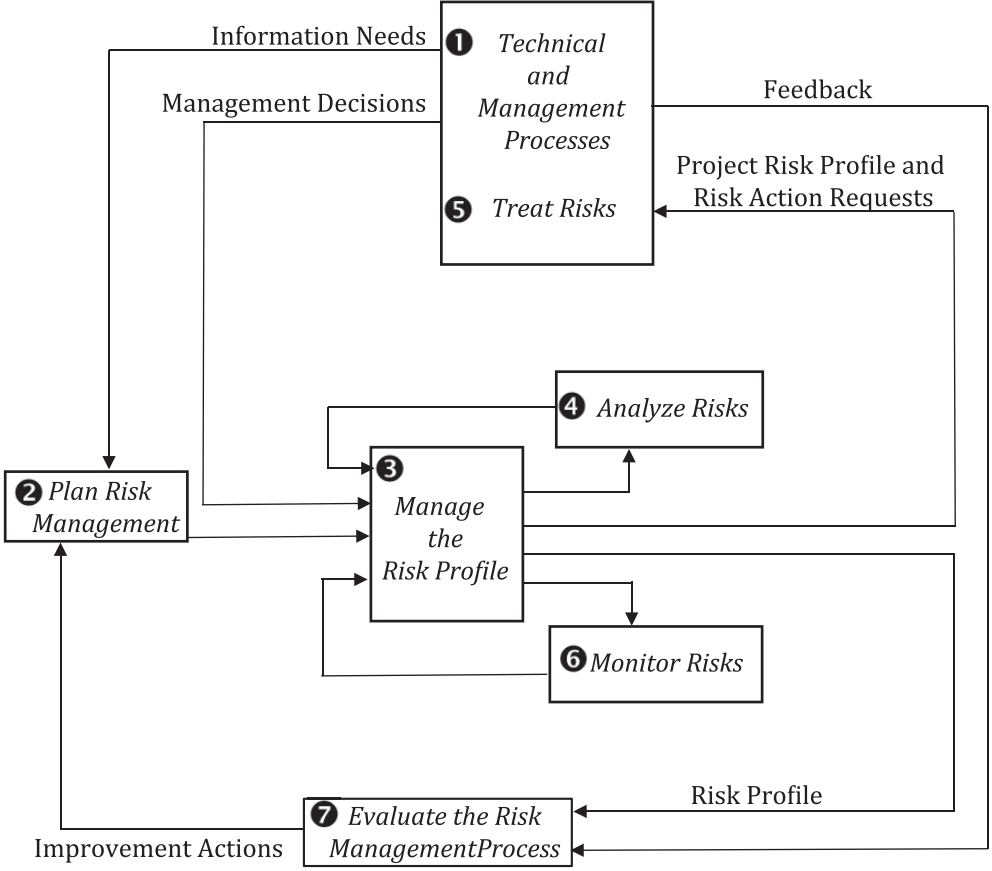
\includegraphics[width=\textwidth]{modelo-processo-gerenciamento-riscos}
	\legend{Fonte: \citeonline{iso16085}}
\end{figure}

Os \textbf{Processos técnicos e de gestão} que envolvem as partes interessadas definem os requisitos de informação (ou seja, as informações que as partes interessadas precisam para tomar decisões informadas envolvendo riscos) que apoiam o processo de gerenciamento de riscos. Esses requisitos de informação são repassados tanto para as atividades de Planejamento da gestão de riscos quanto para Gerenciamento do perfil de risco.

Na atividade de \textbf{Planejamento da gestão de riscos}, são definidas as políticas relativas às diretrizes gerais sob as quais o gerenciamento de riscos será conduzido, os procedimentos a serem usados, as técnicas específicas a serem aplicadas e outros assuntos relevantes ao planejamento de riscos. As informações criadas durante essa atividade devem ser documentadas em um plano de gerenciamento de riscos.

Na atividade de \textbf{Gerenciamento do perfil de risco}, são capturadas as informações sobre o contexto atual e histórico do gerenciamento de riscos e o estado dos riscos. O perfil de risco inclui o total de todos os perfis de risco individuais (ou seja, as informações atuais e históricas sobre um risco individual), que, por sua vez, inclui todos os estados de risco.

As informações do perfil de risco são continuamente atualizadas e mantidas por meio da atividade de \textbf{Análise de riscos}, que identifica os riscos, determina suas probabilidades e consequências, determina suas exposições ao risco e recomenda tratamentos para os riscos considerados acima dos seus limiares de risco. 

As recomendações de \textbf{Tratamento de riscos}, juntamente com o status de outros riscos e seus status de tratamento, são enviadas para a revisão da gerência. A gerência decide qual tratamento de risco será implementado para qualquer risco considerado inaceitável. Planos de tratamento de risco são criados para riscos que necessitam de tratamento. Esses planos são coordenados com outros planos de gerenciamento e outras atividades em andamento. As informações criadas durante essa atividade devem ser documentadas em um plano de tratamento de riscos.

Todos os riscos são continuamente monitorados até que não precisem mais ser rastreados, por exemplo, quando são eliminados, durante a atividade de \textbf{Monitoramento de riscos}. Além disso, novos riscos e fontes de risco são procurados. O processo de gerenciamento de riscos é avaliado para melhorar sua eficácia. Durante a atividade de \textbf{Avaliação do processo de gestão de riscos}, são capturadas informações, incluindo feedback de usuários e outras partes, para melhorar o processo ou a capacidade da organização ou do projeto de gerenciar riscos. Melhorias definidas como resultado da avaliação são implementadas na atividade de Planejamento da gestão de riscos.

O processo de gerenciamento de riscos é aplicado continuamente ao longo do ciclo de vida do produto e é integrado com os outros processos do ciclo de vida. As atividades e tarefas do processo de gerenciamento de riscos interagem com os riscos individuais de maneira iterativa uma vez que o processo de gerenciamento de riscos começa. Por exemplo, na atividade de Análise de riscos, um risco pode ser reavaliado várias vezes durante a realização da avaliação de risco devido ao aumento do conhecimento sobre o risco obtido durante a própria tarefa de avaliação. O processo de gerenciamento de riscos não é um processo que segue de uma fase para a próxima, mas sim um processo iterativo e incremental que é implementado conforme necessário.

%------------------------------------------------------------------------------%

\subsubsection{Modelo do Software Engineering Institute (CMMI)}

\citeonline{wazlawick2019} em Engenharia de Software apresenta o modelo de gerenciamento de riscos do Software Engineering Institute (SEI) e caracteriza da seguinte forma suas seis atividades:

\begin{enumerate}
  \item \textbf{Identificação}: antes que os riscos possam ser tratados, eles precisam ser identificados.
  \item \textbf{Análise}: transforma a lista de riscos potenciais em um documento mais útil para o planejador e o gerente de um projeto, pois, a partir dela, os riscos são priorizados, e o planejador e o gerente podem se concentrar nos riscos mais importantes sem perder tempo com os insignificantes.
  \item \textbf{Planejamento}: o planejamento quanto aos riscos permite ao gerente prevenir problemas, em geral de três formas:
  \begin{enumerate}
    \item planejando e executando planos para reduzir a probabilidade de o risco ocorrer;  
    \item planejando e executando planos para reduzir o impacto do risco, caso ocorra;  
    \item planejando as atividades de recuperação de projeto, caso o risco efetivamente tenha ocorrido.
  \end{enumerate}
  \item \textbf{Rastreamento}: o rastreamento (ou monitoramento) de riscos consiste em avaliar, ao longo do projeto, as propriedades do risco (por exemplo, a probabilidade de ele ocorrer). O rastreamento deve ser baseado em métricas de avaliação de risco.  
  \item \textbf{Controle}: em função de mudanças no status de um risco, alguns planos podem ter que ser executados. Muitas vezes, talvez seja necessário improvisar a resposta ao problema causado pelo risco  
  \item \textbf{Comunicação}: a comunicação é um processo fundamental ao longo de um projeto de software, especialmente em relação à prevenção e ao tratamento de riscos. Assim, não há uma atividade específica de comunicação em riscos, pois se trata de uma prática que permeia todas as outras atividades.
\end{enumerate}
  
%------------------------------------------------------------------------------%

\subsubsection{Modelo do PMBOK}

O PMBOK \cite{PMBOK} possui um dos  processos de gerenciamento de riscos mais conhecidos da área atualmente. Ele é definido em 7 etapas distintas:

\begin{enumerate}
  \item \textbf{Planejar o Gerenciamento dos Riscos}: Processo de definição de como conduzir as atividades de gerenciamento dos riscos de um projeto.

  O principal benefício deste processo é garantir que o grau, o tipo e a visibilidade do gerenciamento dos riscos sejam proporcionais tanto aos riscos como à importância do projeto para a organização e para as outras partes interessadas.  
  
  Deve começar na concepção do projeto e estar concluído no início do projeto. Talvez seja necessário revisitar este processo mais tarde no ciclo de vida do projeto, por exemplo, em uma mudança importante de fase ou se houver mudança significativa no escopo do projeto ou se uma revisão subsequente da eficácia do gerenciamento dos riscos determinar que o processo de Gerenciamento dos Riscos do Projeto exige modificação.

  \item \textbf{Identificar os Riscos}: Processo de identificação dos riscos individuais do projeto, bem como fontes de risco geral do projeto, e de documentar suas características.  
  
  O principal benefício deste processo é a documentação de cada risco de projeto existente e as fontes gerais de riscos do projeto. Também reúne informações para que a equipe do projeto possa responder de forma apropriada aos riscos identificados.  
  
  Todas as partes interessadas do projeto devem ser incentivadas a identificar os riscos individuais do projeto. É especialmente importante envolver a equipe do projeto de modo que ela possa desenvolver e manter um sentido de propriedade e responsabilidade pelos riscos individuais identificados, o nível do risco geral do projeto e as respectivas ações de resposta aos riscos.  

  Na descrição e registro de cada risco do projeto, deve-se usar um formato uniforme para as especificações dos riscos para garantir que cada risco seja compreendido claramente e sem equívocos.

  Identificar os riscos é um processo iterativo, pois novos riscos podem surgir no decorrer do projeto, através de seu ciclo de vida e o nível de risco geral do projeto também pode mudar.

  \item \textbf{Realizar a Análise Qualitativa dos Riscos}: Processo de priorização de riscos individuais do projeto para análise ou ação posterior, através da avaliação de sua probabilidade de ocorrência e impacto, assim como outras características.  
  
  O principal benefício deste processo é que concentra os esforços em riscos de alta prioridade. Este processo é realizado ao longo do projeto.  
  
  Este processo avalia a prioridade dos riscos individuais identificados do projeto utilizando as respectivas probabilidades de ocorrência e o impacto correspondente sobre os objetivos do projeto se os riscos ocorrerem e outros fatores. Essas avaliações são subjetivas, pois baseiam-se em percepções do risco pela equipe do projeto e outras partes interessadas. Portanto, uma avaliação eficaz requer a identificação explícita e o gerenciamento das atitudes dos riscos dos participantes chave no processo. A percepção do risco introduz a parcialidade na avaliação dos riscos identificados; por isso, é preciso estar atento para identificá-los e corrigi- los. Uma avaliação da qualidade das informações disponíveis sobre os riscos individuais do projeto também ajuda a esclarecer a avaliação da importância de cada risco para o projeto.

  \item \textbf{Realizar a Análise Quantitativa dos Riscos}: O processo de analisar numericamente o efeito combinado dos riscos individuais identificados no projeto e outras fontes de incerteza nos objetivos gerais do projeto.  
  
  O principal benefício deste processo é que quantifica a exposição ao risco geral do projeto, e também pode fornecer informações quantitativas adicionais dos riscos para apoio do planejamento de respostas aos mesmos. Este processo não é necessário para todos os projetos.  
  
  Realizar uma análise robusta depende da disponibilidade de dados de alta qualidade sobre os riscos individuais do projeto e outras fontes de incerteza, bem como uma sólida linha de base subjacente do projeto para escopo, cronograma e custo. A análise quantitativa dos riscos geralmente requer software especializado e expertise no desenvolvimento e na interpretação dos modelos de riscos. O uso da análise quantitativa de riscos de um projeto será especificado no plano de gerenciamento dos riscos do projeto.

  \item \textbf{Planejar as Respostas aos Riscos}: O processo de desenvolver alternativas, selecionar estratégias e acordar ações para lidar com a exposição geral de riscos, e também tratar os riscos individuais do projeto.  
  
  O principal benefício deste processo é que identifica formas apropriadas de abordar o risco geral e os riscos individuais do projeto. Este processo também aloca recursos e adiciona atividades em documentos do projeto e no plano de gerenciamento do projeto, conforme necessário.  
  
  As respostas efetivas e apropriadas ao risco podem minimizar ameaças individuais, maximizar oportunidades individuais e reduzir a exposição geral ao risco do projeto. Respostas inadequadas ao risco podem ter o efeito inverso. As respostas planejadas devem ser adequadas à relevância do risco, ter eficácia de custos para atender ao desafio, serem realistas dentro do contexto do projeto, acordados por todas as partes envolvidas e ter um responsável designado.  
  
  Para cada risco, deve-se selecionar a estratégia ou a mescla de estratégias com maior probabilidade de eficácia. Um plano de contingência pode ser desenvolvido para implementação, caso a estratégia selecionada se mostre ineficaz, em parte, ou caso ocorra um risco aceito.

  \item \textbf{Implementar Respostas a Riscos}: Processo de implementar planos acordados de resposta aos riscos.  
  
  O principal benefício deste processo é a garantia de que as respostas acordadas aos riscos sejam executadas conforme planejado a fim de abordar a exposição ao risco geral do projeto, minimizar ameaças individuais e maximizar as oportunidades individuais do projeto. Devida atenção a este processo garante que respostas acordadas são realmente executadas, pois um problema comum com o Gerenciamento dos Riscos é que as equipes empenhem esforços para identificar e analisar riscos e desenvolver respostas, mas nenhuma providência seja tomada para gerenciar os riscos.

  \item \textbf{Monitorar os Riscos}: Processo de monitorar a implementação de planos acordados de resposta aos riscos, acompanhar riscos identificados, identificar e analisar novos riscos, e avaliar a eficácia do processo de risco ao longo do projeto.  
  
  O principal benefício deste processo é que habilita decisões do projeto com base em informações atuais sobre a exposição geral de risco e riscos individuais do projeto.  
  
  Para garantir que a equipe do projeto e as partes interessadas chave estejam cientes do nível atual de exposição ao risco, o trabalho de projeto deve ser constantemente monitorado quanto a riscos individuais novos, alterados, defasados e para as mudanças no nível do risco geral do projeto pela aplicação do processo.
\end{enumerate}

%------------------------------------------------------------------------------%

\section{Métodos ágeis}

O modelo cascata começou a ser definido nos anos 1970 e é considerado o  precursor de todos os ciclos de vida de software. Baseado na filosofia \textit{Big Design Up Front}, ele propõe que antes de qualquer codificação  é necessário realizar um trabalho detalhado de análise e design. O modelo é definido por documentação, determinando se as fases foram concluídas através de revisões ao final de cada uma das etapas \cite{wazlawick2019}. Apesar de sua abordagem estruturada, o modelo enfrenta desafios como a dificuldade de avaliar a qualidade e os riscos do projeto durante o desenvolvimento e a rigidez em lidar com mudanças nos requisitos, pontos que, como apontado por Wazlawick, tornam seu uso impraticável para muitos projetos reais.

Os desafios enfrentados por este modelo preditivo deram origem a ciclos de vida iterativos e incrementais, que abordam melhor as incertezas e as necessidades de adaptação ao longo do projeto. Diferentemente dos métodos preditivos, que se baseiam em planos detalhados para antecipar todas as etapas de um projeto, os métodos iterativos dividem o trabalho em ciclos menores, permitindo revisões frequentes e maior flexibilidade para ajustes \cite{AgileGuide}. Essa abordagem adaptativa é essencial em contextos de alta complexidade e incerteza, onde mudanças nos requisitos são inevitáveis.

No entanto, a principal distinção entre os métodos baseados em planos e os ágeis está no foco. Enquanto os métodos preditivos priorizam o cumprimento do plano inicial, os métodos ágeis enfatizam a entrega contínua de valor ao cliente e a resposta rápida a mudanças. Essa filosofia promove ciclos curtos de desenvolvimento, colaboração constante entre as partes interessadas e feedback contínuo para ajustes ao produto final \cite{AgileGuide}.

A relevância dos métodos ágeis cresceu exponencialmente à medida que organizações perceberam as limitações do modelo preditivo em projetos dinâmicos e complexos. Com a ênfase na adaptação e entrega de valor, os métodos ágeis ganharam destaque em um ambiente onde a velocidade de resposta e a qualidade da entrega são fundamentais para atender às expectativas do mercado e dos clientes.

Em 2001 um grupo de 17 profissionais de software se reuniu em Snowbird, Utah, para discutir formas de melhorar o desenvolvimento de software. Dessa reunião surgiu o Manifesto Ágil, que delineia quatro valores fundamentais e doze princípios que promovem uma abordagem responsiva ao desenvolvimento de software \cite{AgileManifest}. Os quatro valores centrais do Manifesto Ágil são:

\begin{itemize}
  \item Indivíduos e interações mais que processos e ferramentas.
  \item Software funcionando mais que documentação abrangente.
  \item Colaboração com o cliente mais que negociação de contratos.
  \item Responder a mudanças mais que seguir um plano.
\end{itemize}
  
Os princípios do Manifesto enfatizam a entrega contínua de software funcional, a aceitação de mudanças nos requisitos, a colaboração diária entre desenvolvedores e clientes, e a importância de equipes auto-organizadas e motivadas \cite{AgileManifest}. Os doze princípios do Manifesto são:
\begin{itemize}
  \item Nossa maior prioridade é satisfazer o cliente através da entrega contínua e adiantada de software com valor agregado.  
  \item Mudanças nos requisitos são bem-vindas, mesmo tardiamente no desenvolvimento. Processos ágeis tiram vantagem das mudanças visando vantagem competitiva para o cliente.  
  \item Entregar frequentemente software funcionando, de poucas semanas a poucos meses, com preferência à menor escala de tempo.  
  \item Pessoas de negócio e desenvolvedores devem trabalhar diariamente em conjunto por todo o projeto.  
  \item Construa projetos em torno de indivíduos motivados. Dê a eles o ambiente e o suporte necessário e confie neles para fazer o trabalho.  
  \item O método mais eficiente e eficaz de transmitir informações para e entre uma equipe de desenvolvimento é através de conversa face a face.  
  \item Software funcionando é a medida primária de progresso.  
  \item Os processos ágeis promovem desenvolvimento sustentável. Os patrocinadores, desenvolvedores e usuários devem ser capazes de manter um ritmo constante indefinidamente.  
  \item Contínua atenção à excelência técnica e bom design aumenta a agilidade.  
  \item Simplicidade \- a arte de maximizar a quantidade de trabalho não realizado \- é essencial.  
  \item As melhores arquiteturas, requisitos e designs emergem de equipes auto-organizáveis.  
  \item Em intervalos regulares, a equipe reflete sobre como se tornar mais eficaz e então refina e ajusta seu comportamento de acordo.
\end{itemize}

É levantado no Agile Practice Guide \cite{AgileGuide} uma série de diferentes modelos ágeis existentes, cobrindo frameworks, métodos e práticas. Estes são destacados na Figura abaixo.

\begin{figure}[H]
  \centering
	\caption{\label{metodos-ageis}Métodos ágeis}
  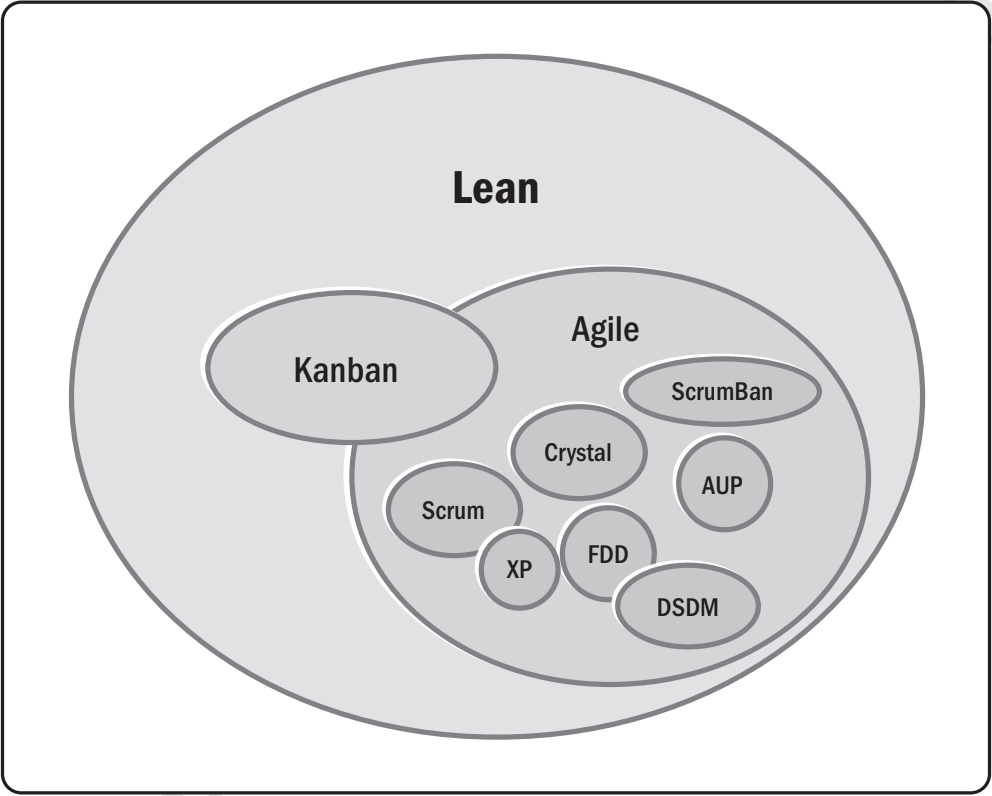
\includegraphics[width=0.6\textwidth]{metodos-ageis}
	\legend{Fonte: Agile Practice Guide \cite{AgileGuide}}
\end{figure}

O \textit{Lean} é definido em \textit{Lean Software Development: An Agile Toolkit} \cite{Poppendieck_Poppendieck_2003} como uma abordagem que visa otimizar processos eliminando desperdícios e adicionando valor de acordo com a percepção do cliente. Entre seus princípios estão a eliminação de desperdícios, que envolve identificar e remover qualquer atividade que não agregue valor ao produto final. Amplificar o aprendizado é essencial, pois o desenvolvimento é um processo de descoberta contínua. Decidir o mais tarde possível permite tomar decisões mais informadas e com base em fatos concretos. A entrega rápida é fundamental para obter feedback contínuo e atender rapidamente às necessidades dos clientes. A equipe deve ser empoderada para tomar decisões técnicas detalhadas, pois eles possuem o conhecimento mais profundo sobre o trabalho. Construir integridade no produto significa assegurar que ele atenda às expectativas do usuário e se mantenha útil ao longo do tempo. Finalmente, ver o todo é crucial para garantir que todas as partes do sistema trabalhem de forma coesa e otimizada, evitando a subotimização de componentes individuais.

\begin{figure}[H]
	\caption{\label{annual-agile-report}Frameworks utilizados pelos respondentes do Agile Report}
  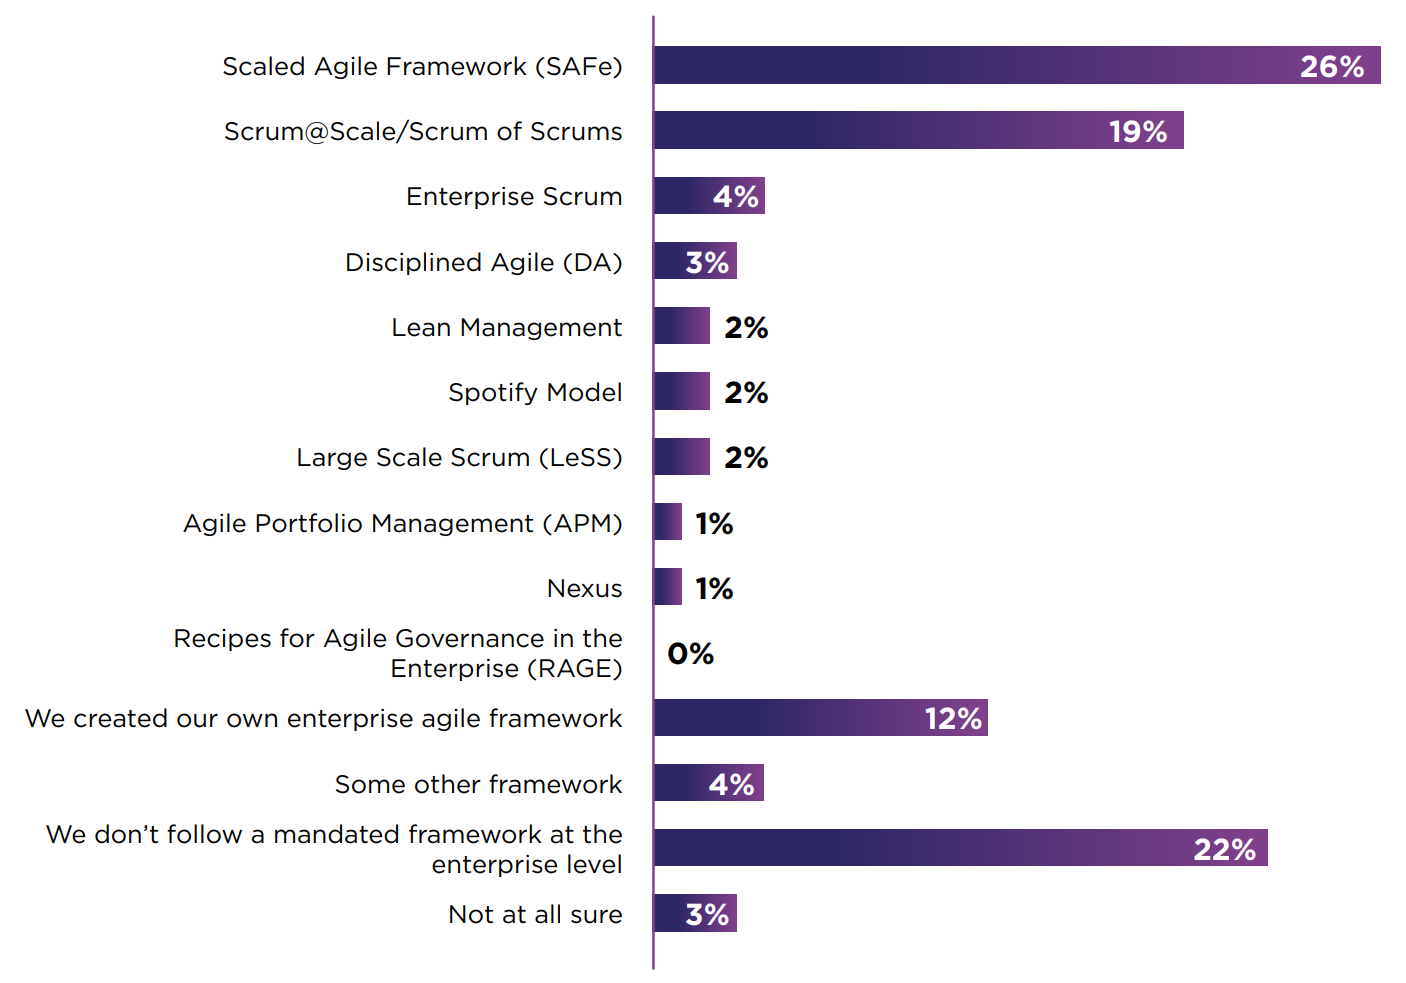
\includegraphics[width=\textwidth]{annual-agile-report}
	\legend{Fonte: 17th State of Agile Report \cite{17_agile_report}}
\end{figure}

Como pode ser observado na Figura 3, segundo o 17th State of Agile Report \cite{17_agile_report}, entre os métodos ágeis mais utilizados em 2023 estão o Scrum e o Scaled Agile Framework (SAFe), definidos como:
\begin{itemize}
  \item \textbf{Scrum}: método ágil de gerenciamento de projetos que visa aumentar a produtividade das equipes de desenvolvimento. Ele não é um processo prescritivo, mas sim um framework que se baseia em três pilares principais: transparência, inspeção e adaptação. A transparência assegura que todos os aspectos importantes do projeto sejam visíveis para os interessados, permitindo que clientes acompanhem o progresso e que desenvolvedores entendam claramente as necessidades do cliente. A inspeção envolve a revisão constante do trabalho realizado para garantir a qualidade e corrigir possíveis desvios. A adaptação permite que o processo de desenvolvimento evolua à medida que novos requisitos são descobertos ou atualizados \cite{wazlawick2019}.
  \item \textbf{Scaled Agile Framework (SAFe)}: framework ágil que visa escalar o desenvolvimento ágil em todos os níveis de uma organização, proporcionando uma base de conhecimento para padrões de trabalho. Baseado em princípios como pensamento sistêmico e preservação de opções em cenários variáveis, o SAFe incentiva a construção incremental com ciclos de aprendizado rápidos e integrados. Adicionalmente, prioriza a limitação de trabalho em progresso, sincronização de planejamento entre domínios e descentralização das tomadas de decisão. Sua abordagem foca em detalhar práticas, papéis e atividades em níveis de portfólio, programa e equipe, organizando a empresa em torno de fluxos de valor contínuo para o cliente \cite{AgileGuide}.
\end{itemize}
  
Apesar das diferenças, Scrum e SAFe compartilham características comuns, como a ênfase na colaboração contínua com o cliente, a entrega frequente de valor em incrementos, a capacidade de adaptação a mudanças e a promoção de equipes auto-organizadas e multifuncionais. Ambos os frameworks incentivam o aprendizado contínuo, a transparência no trabalho e o alinhamento entre as partes interessadas, criando um ambiente que melhora a eficiência, a qualidade e a capacidade de atender às demandas dinâmicas do mercado.

%------------------------------------------------------------------------------%

\subsection{Gestão de riscos em métodos ágeis}

O gerenciamento de riscos em métodos ágeis segue uma abordagem que integra práticas e princípios fundamentais ao processo de desenvolvimento de software inerentemente, sem que haja nenhum procedimento específico para a gestão de riscos \cite{Gold}. Práticas como retrospectivas, dailies e sprints com entregas incrementais desempenham papel fundamental na identificação e mitigação de riscos, que acabam por acontecer de forma implícita. Essa forma implícita ocorre porque o processo ágil favorece ciclos curtos de feedback, transparência e colaboração contínua entre as partes interessadas, o que permite identificar problemas ou ameaças de forma rápida e iterativa. Assim, os riscos são tratados à medida que surgem, promovendo ajustes frequentes ao longo do projeto.

Em outra perspectiva pode-se considerar que o gerenciamento de riscos tem sido negligenciado ou parcialmente suportado em métodos ágeis, mesmo com o aumento da importância do gerenciamento de riscos entre as organizações, já que os riscos podem surgir ao longo do ciclo de vida do projeto e não existe nenhuma ação específica para evitar estes riscos \cite{LopesSamueldeSouza2022ARMF}. Pensando na prática, o Scrum, por exemplo, tem uma seção para quaisquer 'impedimentos' do projeto, que são ocorrências que possam impedir a equipe de funcionar de maneira eficaz. Do ponto de vista do gerenciamento de riscos, os impedimentos do projeto são problemas, riscos que ocorreram \cite{Gold}. Havendo um processo estruturado de gestão de riscos, não seria necessário tratar o problema, pois o risco que o gera poderia ter sido identificado e resolvido, antes de se tornar um problema.

\citeonline{LopesSamueldeSouza2022ARMF} vêem que devido à receptividade às mudanças no método ágil, vários projetos apresentam incertezas e riscos, e no formato atualmente, vários riscos permanecem desconhecidos porque são ignorados ao longo do ciclo de vida do projeto. Estes riscos podem ser gerenciados por meio de processos tradicionais de gerenciamento de riscos, desde que sejam adaptados ao contexto do desenvolvimento ágil.

Na pesquisa de \citeonline{Gold} foram identificados certos fatores que aumentam a eficácia do gerenciamento de riscos, um deles é a aplicação de um framework de gerenciamento de riscos (identificação ágil de riscos, avaliação ágil de riscos, resposta ágil a riscos, revisão e monitoramento ágeis de riscos). Foi visto pelos entrevistados que a aplicação dessas etapas de gerenciamento de riscos tem grande influência positiva nos resultados do projeto, mostrando que o uso das práticas de gerenciamento de riscos neste cenário proporcionam resultados mais benéficos do que limitações. Foram avaliados os seguintes benefícios da aplicação do gerenciamento de riscos a projetos Scrum \cite{Gold}:
\begin{itemize}
  \item Riscos e problemas ocorrem durante os projetos; uma equipe pode escolher ser reativa ou proativa em relação a esses riscos e problemas. O gerenciamento proativo de riscos durante todo o projeto é significativo para o sucesso do projeto e influencia positivamente o resultado do projeto.
  \item O gerenciamento de riscos ajuda a fornecer uma visão geral dos possíveis riscos que podem ser encontrados durante um projeto e a se preparar adequadamente para esses riscos.
  \item Embora o Scrum já seja orientado a riscos devido à sua natureza ágil, a aplicação de um processo de gerenciamento de riscos reforça ainda mais esse método, melhorando sua entrega em relação aos seus fatores críticos de sucesso de tempo, custo e qualidade.
\end{itemize}

%------------------------------------------------------------------------------%

\section{Gamificação}

Definida como a aplicação de elementos de design de jogos fora do contexto de jogos, a gamificação visa aumentar o engajamento, a motivação e, consequentemente, os resultados dos indivíduos na atividade gamificada \cite{GARCIA201721}. Segundo \citeonline{Fardo_2013}, “a gamificação é um fenômeno com muitas potencialidades, pois a linguagem e metodologia dos games são bastante populares, eficazes na resolução de problemas [...] e aceitas naturalmente pelas atuais gerações.”, mostrando a gamificação como uma estratégia importante a ser explorada.  

Aplicações da gamificação são amplas e variadas. Na educação, como observado por \citeonline{Alomari}, a gamificação pode transformar ambientes de aprendizagem ao tornar o estudo mais interativo e motivador. No marketing, ela pode aumentar a fidelidade dos clientes e a interação com a marca. No campo da saúde, a gamificação pode incentivar comportamentos saudáveis, como a prática de exercícios físicos e a adesão a tratamentos médicos. Ainda, como visto por \citeonline{Caponetto}, o uso da gamificação se mostra eficaz para alcançar objetivos transversais, como promover abordagens participativas e a colaboração entre pares, incentivar o aprendizado autodirigido e explorar a criatividade.

A gamificação envolve um processo de definição do ponto de vista de um designer de jogos, transformando uma tarefa em uma experiência que concentre o foco do participante para a resolução de um problema \cite{Fardo_2013}. Ela é criada a partir da integração de elementos comuns nos jogos, que, como identificado por \citeonline{Alomari}, podem envolver: sistemas de pontuação, badges, rankeamento (leaderboard), níveis, recompensas, barras de progresso, desafios, feedback e avatares. \citeonline{Alomari} identifica os elementos típicos abaixo como as mais usadas e as caracteriza da seguinte forma:
\begin{itemize}
  \item \textbf{Points}: Pontos são definidos como valores numéricos que representam uma avaliação do indivíduo. Esta técnica fornece um feedback sobre o progresso do indivíduo e pode aumentar a sua motivação.
  
  \item \textbf{Badges}: Badges são um maneira visual de representar as conquistas alcançadas pelo indivíduo na atividade. Assim como os pontos, ela impacta positivamente a motivação. Esta representação visual tem ênfase em melhorar a performance dos participantes.
  
  \item \textbf{Leaderboard}: Leaderboard são uma exibição do ranking dos participantes. Ele permite que o participante veja sua performance e a de seus colegas, o que resulta em um estímulo individual para engajar mais na atividade.
\end{itemize}

Pode ser observado na Figura 4 um exemplo do uso da técnica PBL (Points, Badges, Leaderboard) no aplicativo para aprendizado de línguas Duolingo.

\begin{figure}[H]
	\caption{\label{duolingo}Sistema PBL no Duolingo}
  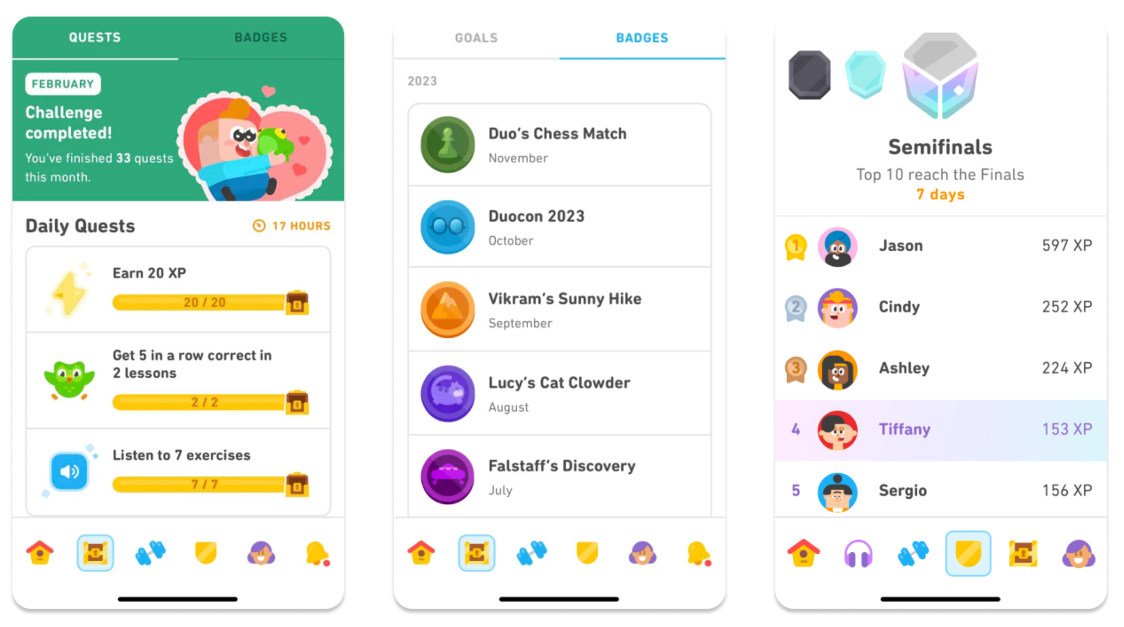
\includegraphics[width=\textwidth]{duolingo}
	\legend{Fonte: Duolingo, Inc.}
\end{figure}

Para poder então criar um processo gamificado para uma atividade, \citeonline{GARCIA201721} identificam uma sequência bem definida de passos:

\renewcommand{\arraystretch}{1.3}

\begin{table}[h!]
  \caption{Metodologia para desenvolvimento de sistemas gamificados}
  \centering
  \resizebox{\textwidth}{!}{
  \begin{tabular}{|p{9cm}|p{6cm}|}
  \hline
  \textbf{Atividade} & \textbf{Descrição} \\ \hline
  \textbf{Identificação dos objetivos da gamificação} \newline 
  Tarefas: \newline 
  1.1 Definir o cenário atual \newline 
  1.2 Definir o cenário-alvo \newline 
  1.3 Estabelecer a missão SMART 
  & Os objetivos do programa de gamificação são definidos, juntamente com os indicadores correspondentes que devem avaliar o cumprimento dos objetivos. \\ \hline

  \textbf{Análise dos jogadores} \newline 
  Tarefas: \newline 
  2.1 Identificar a cultura organizacional e tipos de jogadores \newline 
  2.2 Coletar informações demográficas e psicográficas de todos os jogadores e adicionar isso ao perfil. 
  & Cada jogador é analisado em seu contexto para alinhar os perfis dos jogadores com os objetivos da gamificação. \\ \hline

  \textbf{Definição do escopo da gamificação e estudo de viabilidade} \newline 
  Tarefas: \newline 
  3.1 Estabelecer o escopo, motivadores, tipo de jogo (colaborativo, competitivo, individual) e diferentes possíveis soluções. \newline 
  3.2 Conduzir análise de viabilidade para cada alternativa e escolher a solução. 
  & Para definir o escopo da gamificação (cobertura do ciclo de vida do software e motivadores intrínsecos/extrínsecos do jogo) e conduzir um estudo de viabilidade (econômica, técnica, operacional e legal), para escolher a melhor solução. \\ \hline

  \textbf{Análise e design do jogo} \newline 
  Tarefas: \newline 
  4.1 Escolher os componentes do jogo \newline 
  4.2 Escolher as mecânicas do jogo \newline 
  4.3 Estabelecer a economia do jogo \newline 
  4.4 Estabelecer a dinâmica do jogo (regras) \newline 
  4.5 Estabelecer a estética do jogo \newline 
  4.6 Elaborar os casos de uso do jogo 
  & O principal resultado desta atividade é o conjunto de requisitos (casos de uso do jogo) da ferramenta de software em que o jogo está, e automatiza o jogo e seus elementos. \\ \hline
  
  \textbf{Desenvolvimento da plataforma gamificada} \newline 
  Tarefas para cada sprint: \newline 
  5.1 Gestão da Sprint \newline 
  5.2 Desenvolvimento da Sprint (Preparação, Desenvolvimento, Teste) 
  & Desenvolvimento de software da plataforma gamificada para SE a partir dos casos de uso do jogo. \\ \hline
  
  \textbf{Gerenciamento, monitoramento e medição} \newline 
  Tarefas: \newline 
  6.1 Coletar valores dos indicadores a partir dos logs de execução \newline 
  6.2 Analisar os indicadores e avaliar o cumprimento dos objetivos de negócios \newline 
  6.3 Desenvolver planos de ação para melhorar o sistema gamificado 
  & A plataforma gamificada é periodicamente monitorada para analisar o desempenho e o alcance dos objetivos de negócios. Quando são detectados desvios, planos de ação são desenvolvidos para refinar ou incluir no jogo os elementos necessários (componentes, mecânicas, dinâmica, estética). \\ \hline
  \end{tabular}
  }
  \label{tab:gamificacao}
  \legend{Fonte: Adaptado de \cite{GARCIA201721}}
\end{table}

%------------------------------------------------------------------------------%

\chapter{Estado da arte} % Trabalhos parecidos com os que eu vou desenvolver

A fim de levantar o estado da arte, foi realizada uma replicação e atualização do estudo conduzido por \citeonline{garcia2023agreed} em seu trabalho de mestrado de Mapeamento Sistemático de Literatura (MSL). Nesta replicação as diferenças foram a realização da análise apenas de estudos publicados, analisando estudos publicado a partir de 2021, posteriormente ao mapeamento original, e a não aplicação da técnica de Snowballing no ciclo final.

Assim como no mapeamento original, o MSL foi desenvolvido com o objetivo de analisar a integração de práticas explícitas de gestão de risco em métodos ágeis. Para isso, foram seguidos os procedimentos definidos por \citeonline{PETERSEN20151} e \citeonline{Petersen}, garantindo a aplicação de uma abordagem sistemática e rigorosa na condução da pesquisa.

\section{Protocolo de pesquisa}

A questão geral de pesquisa foi definida como: “Como as organizações de software integram práticas explícitas de gerenciamento de riscos em métodos ágeis?” e esta foi dividida em quatro questões de análise detalhada, conforme apresentada na tabela abaixo.

\begin{table}[h!]
  \caption{Perguntas de pesquisa do MSL}
  \centering
  \begin{tabular}{|c|p{10cm}|}
  \hline
  \textbf{Pergunta} & \textbf{Descrição} \\ \hline
  Q1 & Qual contexto de uso de práticas de gestão de riscos nos métodos ágeis? \\ \hline
  Q2 & Quais práticas de gestão de riscos são introduzidas nos métodos ágeis? \\ \hline
  Q3 & Quais tipos de riscos são gerenciados? \\ \hline
  Q4 & Quais os resultados da introdução de práticas explícitas de gestão de riscos nos métodos ágeis? \\ \hline
  \end{tabular}
  \label{tab:perguntas-msl}
\end{table}

A Tabela~\ref{tab:picoc} \cite{kitchenham2007guidelines} mostra os critérios e o escopo da estrutura da pergunta de pesquisa, que é a estrutura de População, Intervenção, Comparação, Resultados e Contexto (PICOC).

\begin{table}[h!]
  \centering
  \caption{Descrição dos elementos PICOC da Pesquisa}
  \begin{tabular}{|p{3cm}|p{12cm}|}
  \hline
  \textbf{Critérios} & \textbf{Descrição} \\ \hline
  População \newline Intervenção \newline Comparação \newline Resultado \newline Contexto 
  & Organizações de software \newline Aplicação da gerência de riscos \newline Não se aplica (N/A) \newline Se a qualidade do produto, prazo de entrega, etc foram impactados \newline Utilização de métodos ágeis \\ \hline
  \end{tabular}
  \label{tab:picoc}
\end{table}

A comparação é definida como “N/A” por se tratar de um mapeamento sistemático.

%------------------------------------------------------------------------------%

\subsection{String de busca e fontes de pesquisa}

A string de busca foi aplicada nas bibliotecas digitais IEEEXplore, ACM Digital Library e Scopus, devido à sua relevância para a área de engenharia de software. A string de busca foi adaptada à sintaxe específica de cada biblioteca e aplicada aos campos de título e resumos. A pesquisa foi realizada em setembro de 2024.

\begin{table}[h!]
  \centering
  \begin{tabular}{|p{15cm}|}
  \hline
  “risk” AND (“agile” OR “scrum” OR “xp” OR “extreme programming” OR “lean” OR “kanban” OR “scrumban” OR “fdd” OR “feature driven development” OR “crystal” OR “iterative development”) AND “software” \\ \hline
  \end{tabular}
  \label{tab:consulta-pesquisa}
\end{table}
  
Como não é possível realizar a pesquisa em todas as bibliotecas digitais usando a string de busca no mesmo formato, foram necessárias adaptações específicas da string de pesquisa para cada biblioteca digital, conforme descrito no Apêndice A.

%------------------------------------------------------------------------------%

\section{Critérios de inclusão e exclusão}

Com base na questão de pesquisa principal, os seguintes critérios de inclusão e exclusão foram definidos. Para além do estudo original, o critério de inclusão 4 foi adicionado, para o mapeamento de apenas estudos publicados após o fim do mapeamento original.

\begin{table}[h!]
  \centering
  \caption{Critérios de inclusão}
  \begin{tabular}{|c|l|}
  \hline
  \textbf{Critério} & \textbf{Descrição} \\ \hline
  IC1 & Estudos primários revisados por pares \\ \hline
  IC2 & Escrito em inglês \\ \hline
  IC3 & Trabalhos completos com pelo menos 4 páginas \\ \hline
  IC4 & Trabalhos publicado a partir de 2021 \\ \hline
  \end{tabular}
\end{table}
  
\begin{table}[h!]
  \centering
  \caption{Critérios de exclusão}
  \begin{tabular}{|c|l|}
  \hline
  \textbf{Critério} & \textbf{Descrição} \\ \hline
  EC1 & Trabalho/proposta teórica não aplicada empiricamente \\ \hline
  EC2 & Estudos duplicados \\ \hline
  EC3 & Texto completo indisponível \\ \hline
  EC4 & Não focado no desenvolvimento de software \\ \hline
  \end{tabular}
\end{table}

%------------------------------------------------------------------------------%
\section{Processo de seleção}

A seleção dos estudos foi realizada em três ciclos, conforme Figura 5.

\begin{figure}[H]
	\caption{\label{numero-estudos-ciclo}Modelo de processo de gerenciamento de riscos}
  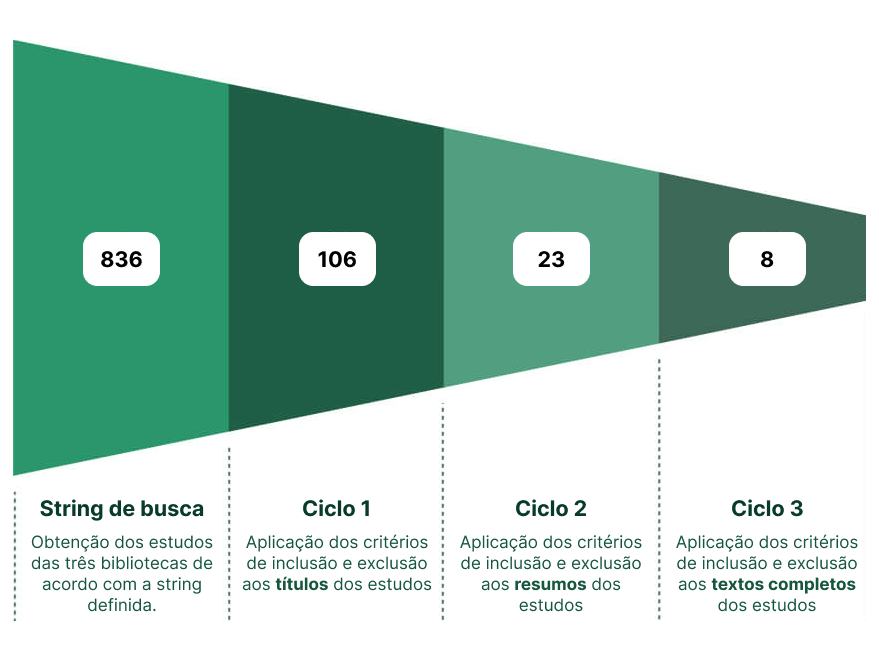
\includegraphics[width=\textwidth]{numero-estudos-ciclo}
	\legend{Fonte: Autora (2024)}
\end{figure}

\begin{itemize}
  \item Para iniciar os ciclos, a string de busca foi aplicada às bibliotecas digitais, onde se obteve 836 estudos primários que foram submetidos à próxima etapa.
  \item No ciclo 1, a lista de estudos anterior foi submetida aos critérios de inclusão e exclusão em seus títulos e a nova seleção resultou em 106 estudos selecionados.
  \item No ciclo 2, a lista de estudos anterior foi submetida aos critérios de inclusão e exclusão em seus resumos e a nova seleção resultou em 23 estudos selecionados.
  \item No ciclo 3, a lista de estudos anterior foi submetida aos critérios de inclusão e exclusão em seus textos completos e esta última e final seleção resultou em 8 estudos selecionados.
\end{itemize}

\begin{table}[h!]
  \centering
  \caption{Resultados por biblioteca digital e ciclo}
  \begin{tabular}{|c|c|c|c|c|}
  \hline
  \textbf{Biblioteca} & \textbf{Total} & \textbf{Ciclo 1} & \textbf{Ciclo 2} & \textbf{Ciclo 3} \\ \hline
  ACM & 185 & 29 & 4 & 1 \\ \hline
  Scopus & 304 & 51 & 14 & 5 \\ \hline
  IEEE Xplore & 347 & 26 & 5 & 2 \\ \hline
  Todos & 836 & 106 & 23 & 8 \\ \hline
  \end{tabular}
\end{table}
  
%------------------------------------------------------------------------------%

\section{Extração dos dados}

Os dados coletados dos estudos primários selecionados são apresentados e analisados de acordo com cada questão de análise pré-definida. Os dados brutos extraídos estão disponíveis em: \href{https://docs.google.com/spreadsheets/d/1YY_yjyBefJ3ZmnEY38TM_LnZLoJcKhrw_q0BdEvqx2E/edit?gid=1276800509#gid=1276800509}{MSL público}. Uma síntese do DEF está descrita na Tabela~\ref{sintese}.

\begin{table}[h!]
  \centering
  \caption{Síntese do DEF}
  \begin{tabular}{|p{2.4cm}|c|p{9.5cm}|}
  \hline
  \textbf{Questão de pesquisa} & \textbf{Identificador} & \textbf{Descrição} \\ \hline
  Q1 & Q1.1 & Contexto de aplicação do estudo \\ \hline
  Q1 & Q1.2 & Método ágil utilizado/impactado \\ \hline
  Q1 & Q1.3 & Tipo de validação do estudo \\ \hline
  Q1 & Q1.4 & Número de projetos que o estudo foi aplicado \\ \hline
  Q2 & Q2.1 & Lista/descrição das práticas propostas \\ \hline
  Q2 & Q2.2 & Processo de gerenciamento de risco impactado pelas práticas propostas \\ \hline
  Q3 & Q3.1 & Riscos enfrentados nos projetos \\ \hline
  Q4 & Q4.1 & Síntese do resultado dos estudos empíricos \\ \hline
  \end{tabular}
  \label{sintese}
\end{table}

\textbf{Q1. Qual é o contexto de uso das práticas de gestão de risco em métodos ágeis?}

Na Tabela~\ref{contexto} é possível observar a resposta direta de cada uma dos seccionamentos desta pergunta.

\begin{table}[h!]
  \centering
  \caption{Contexto de uso}
  \begin{tabular}{|c|l|l|}
  \hline
  \textbf{Questão} & \multicolumn{2}{c|}{\textbf{Extracted data}} \\ \hline
  \multirow{2}{*}{Q1.1 - Ambiente} & Indústria & S1, S2, S3, S4, S6, S8 \\ \cline{2-3}
                                  & Academia  & S5, S7 \\ \hline
  \multirow{6}{*}{Q1.2 - Método ágil} & Scrum   & S3, S5 \\ \cline{2-3}
                                     & XP      & S3 \\ \cline{2-3}
                                     & DAD     & S6 \\ \cline{2-3}
                                     & SAFe    & S6 \\ \cline{2-3}
                                     & Não definido & S1, S2, S4, S7, S8 \\ \hline
  \multirow{3}{*}{Q1.3 - Tipo}        & Estudo de caso & S3, S4, S6, S8 \\ \cline{2-3}
                                     & Experimento    & S1, S2, S5 \\ \cline{2-3}
                                     & Survey         & S7 \\ \hline
  \multirow{2}{*}{Q1.4 - Instâncias}  & Exatamente 1   & S1, S3, S7, S8 \\ \cline{2-3}
                                     & Exatamente 2   & S2, S4, S5, S6 \\ \hline
  \end{tabular}
  \label{contexto}
  \end{table}

Os estudos selecionados foram conduzidos em dois ambientes distintos (Q2.1): indústria de software e academia. Dos estudos analisados, 75\% foram realizados em organizações de desenvolvimento de software, enquanto 25\% foram conduzidos em ambiente acadêmico.

Quanto aos métodos ágeis adotados (Q2.2), Scrum foi mencionado em 2 estudos, XP, DAD e SAFe em 1 estudo cada. Além disso, de forma maior, 4 estudos não mencionaram nenhum método ágil específico.

Em relação ao tipo de estudo empírico (Q2.3), metade dos estudos utilizaram estudos de caso, 37\% realizaram experimentos e 13\% aplicaram surveys. Observa-se que, na indústria, predominam os estudos de caso, como observado no mapeamento original.
O número de projetos em que o estudo foi aplicado ficou entre apenas 1 e 2, divididos de forma igual, 50\% dos estudos aplicados em apenas 1 organização e 50\% aplicaram em 2 organizações.

\textbf{Q2. Quais práticas de gerenciamento de risco são introduzidas nos métodos ágeis?}

Assim como observado no mapeamento original, duas estratégias diferentes foram adotadas pelos estudos para integrar a gestão de riscos aos métodos ágeis: usar as práticas ágeis existentes ou introduzir novas práticas de gestão de riscos.

Os estudos S2 e S6 adotaram a primeira estratégia. Sendo que em S2 são incentivadas prioritariamente as práticas Daily meeting, Increment, Prototype, Product backlog, Sprint planning, Sprint backlog, Product backlog refinement meeting. Além disso, em S2 é sugerida uma prática da segunda estratégia, ao definir uma “Risk weekly meeting”.

Adotando a segunda estratégia, os outros estudos primários criaram novas práticas ágeis ou introduziram práticas tradicionais adaptadas em métodos ágeis para melhorar o gerenciamento de riscos. O Apêndice C apresenta as práticas de gerenciamento de risco introduzidas, agrupadas pela prática ágil existente impactada (quando aplicável). Alguns exemplos de práticas são descritos abaixo.

Em S1 é instituído o RM3 que é composto por três processos principais: análise de complexidade do projeto, análise de riscos e monitoramento e controle de riscos. Onde em (1) Utiliza-se a Matriz de Complexidade, uma ferramenta qualitativa para avaliar objetivamente os fatores de complexidade e seu impacto; (2) Análise de Riscos: Identifica todos os riscos, tanto negativos quanto positivos, com base nos pressupostos e restrições do projeto. Utiliza a Exposição ao Risco como medida quantitativa para avaliar e priorizar os riscos; (3) Monitoramento e Controle de Riscos: Aplica ações de resposta ao risco e monitora os riscos identificados, atualizando-os conforme necessário. Este processo inclui monitorar e tratar riscos residuais, identificar novos riscos e avaliar a eficácia das respostas. Além disso, atualiza os ativos dos processos organizacionais, como modelos de gestão de riscos e lições aprendidas, beneficiando futuros projetos.

No estudo S3, um backlog específico para riscos é adicionado aos produtos da metodologia para registrar e gerenciar todos os riscos identificados. Além das tarefas do Scrum, as tarefas de gestão de riscos em cada sprint são realizadas em três passos: Planejamento (Identificar e registrar todos os riscos no backlog), Aplicação de Estratégia (Priorizar os riscos com base em fatores de prioridade, inserir os riscos de maior prioridade no ciclo de iteração do Scrum, e aplicar a estratégia apropriada para cada risco.) e Supervisão e Controle (Monitorar a eliminação dos riscos e assegurar que a estratégia está sendo eficaz.) No final de cada sprint, avalia-se a harmonia entre as estratégias aplicadas e os riscos. Caso novos riscos sejam identificados ou riscos existentes persistam, eles retornam ao backlog de riscos para análise e tratamento em sprints futuras.

Em S8, é descrito o problema de minimização de perdas por riscos no processo de design de software definido considerando Vetor de Variáveis de Decisão. Onde a partir da Probabilidade de ocorrência do risco para o i-ésimo recurso, o Valor das perdas por unidade do i-ésimo recurso associado à ocorrência do risco, o Número do recurso do projeto é feito o Cálculo da Estimativa Total de Risco (R). E a Função Objetivo: Determinar a quantidade de cada recurso a ser alocado no projeto, de forma que a função objetivo  \( F(x) \) (o custo de compensação das consequências dos riscos) seja minimizada.

\textbf{Q3. Que tipos de riscos são gerenciados?}

Os estudos primários selecionados identificam um total de 97 riscos. Assim como no mapeamento original foram agrupados por meio de uma taxonomia de riscos que fornece três classes de riscos, seus elementos e atributos. Todos os riscos relatados nos estudos primários selecionados foram coletados, classificados de acordo com a taxonomia e resumidos no Apêndice D. A lista completa de riscos, suas fontes e as classificações escolhidas está disponível em: \href{https://docs.google.com/spreadsheets/d/1YY_yjyBefJ3ZmnEY38TM_LnZLoJcKhrw_q0BdEvqx2E/edit?usp=drivesdk}{link}.

Apenas 5 dos 8 estudos listaram de forma explícita os riscos enfrentados nos projetos. Deste grupo, o estudo primário que relatou o maior número de riscos foi S6, com um total de 63 riscos, tendo alta distribuição entre as diferentes classes, elementos e atributos, como é possível observar na Figura 6.

\begin{figure}[H]
	\caption{\label{dist-contagem-classe-atributo}Distribuição de contagem por classe e atributo de S6}
  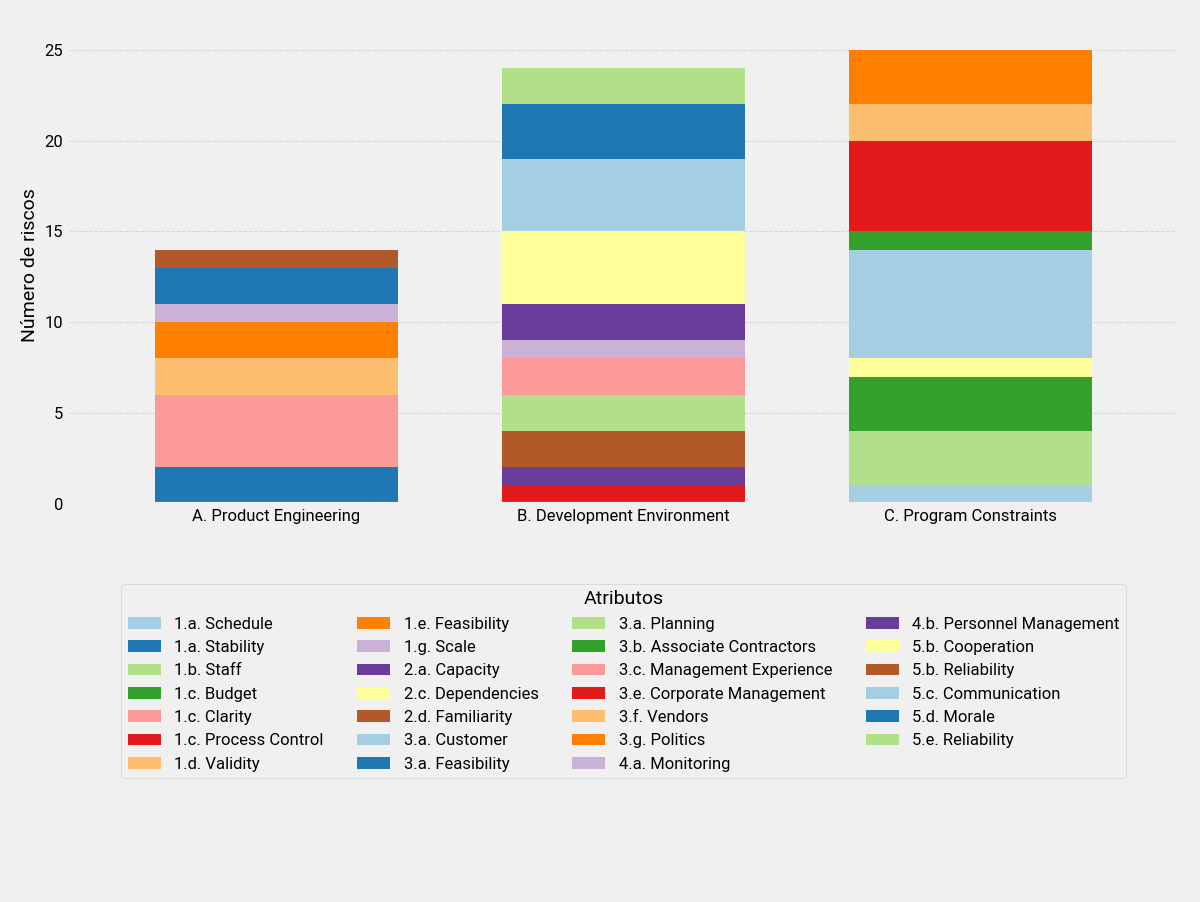
\includegraphics[width=\textwidth]{dist-contagem-classe-atributo}
	\legend{Fonte: Autora (2024)}
\end{figure}

O atributo com maior frequência de riscos foram “Schedule”, da classe “Program Constraints”, identificado em 4 dos estudos primários. Em sequência “Staff”, da classe “Product Engineering”, “Communication”, da classe “Development Environment” e “Stability”,  “Clarity”, “Validity” e  “Feasibility”, da classe “Product Engineering”, obtiveram 3 ocorrências cada.

O elemento com maior número de ocorrências de riscos foi ”Resources”, registrado em 4 estudos primários. “Product Engineering” e “Program Constraints” foram as  classes que apresentaram o maior número de ocorrências, ambas com registros em 4 estudos.

\textbf{Q4. Quais são os resultados da introdução de práticas explícitas de gerenciamento de riscos em métodos ágeis?}

Todos os estudos selecionados relatam impactos positivos da introdução de práticas explícitas de gerenciamento de riscos, mas 4 estudos (50\%) [S2, S3, S6, S8] destacaram explicitamente impactos positivos sem comprometer a agilidade dos métodos ágeis.

Em S1 do ponto de vista financeiro, de escopo e de prazos, o projeto foi bem-sucedido e atendeu às expectativas da equipe. Houve menos tempo gasto em atividades desnecessárias, o que permitiu mais foco e ausência de riscos inesperados. Os recursos foram liberados conforme planejado, garantindo a qualidade das entregas e continuidade do trabalho da equipe em outros projetos. Foi aplicado um questionário para medir a satisfação da equipe, do cliente e das partes interessadas com o uso do RM3, e o resultado foi muito positivo,  demonstrando preferência pelo RM3 em relação ao método anterior.

No estudo S4, aplicado em projetos com mais de 5 mil horas de duração de 5 a 10 meses para serem concluídos, o uso do framework gerou um aumento positivo na reação média aos riscos, com uma taxa de melhoria de cerca de 49\%.

Em S5 os resultados indicam um aumento significativo no conhecimento sobre gestão de riscos ao utilizar o jogo, destacando seu valor educacional e eficácia como ferramenta de apoio ao ensino. Houve uma melhoria de 85\% nas respostas do questionário do Grupo AAS, com apenas 15\% dos participantes mantendo as mesmas respostas iniciais.

Na análise de S6 o mapeamento teórico demonstra como os frameworks escaláveis de ágil — DAD e SAFe — podem potencialmente eliminar ou mitigar os riscos de projetos de software no contexto de desenvolvimento global.

Em S2 o uso da ferramenta Rm4Am aumentou a média do índice de resposta a riscos em de 63\% no Projeto A e 40\% no Projeto B, indicando que a ferramenta auxiliou os participantes na formulação de planos de resposta a riscos mais eficazes.

\section{Discussão}

Como também identificado no mapeamento original, a maioria dos estudos foram feitos na indústria, mostrando o potencial impacto positivo das ações de gestão de risco para esta área. Havendo também 50\% dos estudos relatando impactos positivos sem comprometer a agilidade dos métodos ágeis. Além disso, estudos de caso são predominantes na indústria, enquanto experimentos e surveys têm menor representatividade, mostrando uma tendência de abordagem empírica para avaliar os contextos de uso dessas práticas.

As práticas de gestão de riscos nos métodos ágeis se dividem em duas estratégias principais: o uso das práticas ágeis já existentes e a introdução de novas práticas adaptadas. Por exemplo, práticas como reuniões diárias e planejamento de sprints foram aproveitadas para integrar a gestão de riscos, além da inclusão de uma reunião semanal dedicada a riscos. Por outro lado, foi observado também a ideia de criação de um backlog específico para riscos, ou ainda do uso de métodos quantitativos para minimizar perdas, como o cálculo de estimativa total de risco e alocação de recursos.

Os tipos de riscos gerenciados foram classificados em uma grande variedade de atributos em todas as classes. Estudos como S6, que identificou 63 riscos, mostram a complexidade e a amplitude dos desafios enfrentados, destacando a necessidade de métodos estruturados e adaptados para lidar com essas incertezas no desenvolvimento ágil.

Por fim, os resultados indicam impactos positivos significativos na introdução de práticas explícitas de gestão de riscos, sem comprometer a agilidade dos métodos ágeis. Exemplos incluem a melhoria na eficiência e qualidade das entregas, maior conhecimento sobre gestão de riscos e aumento da eficácia no tratamento de riscos com ferramentas específicas, como Rm4Am. Esses resultados reforçam a relevância de integrar práticas de gestão de riscos aos métodos ágeis para alcançar maior sucesso nos projetos.


\subsection{Ameaças à validade}

As mesmas ameaças à validade avaliadas no mapeamento original também estão presentes nesta replicação, como o risco de buscas incompletas, a limitação no número de estudos analisados, a tendência de publicação de resultados positivos e a qualidade empírica limitada de muitos dos estudos incluídos. Ademais, a técnica de Snowballing não foi aplicada nesta replicação, o que impossibilitou a identificação de estudos adicionais e pode ter levado à omissão de trabalhos relevantes. Por fim, como este estudo é uma replicação, eventuais problemas não identificados na pesquisa original também foram reproduzidos, o que pode impactar os resultados e conclusões deste trabalho.


%------------------------------------------------------------------------------%
%------------------------------------------------------------------------------%

\chapter{Proposta}

Seguindo o framework de gamificação em engenharia de software proposto por \citeonline{GARCIA201721}, nas seções seguintes serão apresentadas as atividades realizadas para o desenvolvimento da dinâmica gamificação para identificação de riscos em meios ágeis. O framework prevê as seguinte etapas para esta definição:

\begin{enumerate}
  \item Identificação os objetivos da gamificação  
  \item Análise dos jogadores  
  \item Definição do escopo da gamificação e estudo de viabilidade  
  \item Análise e design do jogo  
  \item Desenvolvimento da plataforma gamificada  
  \item Gerenciamento, monitoramento e medição
\end{enumerate}

\section{Identificação dos objetivos da gamificação}

A primeira etapa do framework busca estabelecer um conjunto de objetivos para a gamificação, sendo que isto deve ser feito examinando o cenário atual e o desejado, identificando situações que podem ser aprimoradas por meio da aplicação da gamificação e como essas melhorias podem ocorrer. Por fim, estes objetivos devem ser convertidos em metas SMART para medir as melhorias alcançadas. Preferencialmente métricas e indicadores quantitativos devem ser definidos, entretanto nem isto é viável, especialmente em organizações com sistemas de medição inexistentes ou imaturos.

\begin{enumerate}
  \item \textbf{Cenário atual}: Equipes ágeis operam em modelos onde o gerenciamento de riscos é implícito, sem etapas estruturadas ou práticas específicas para identificar e analisar riscos. Essa ausência de um gerenciamento de riscos explícito pode resultar na negligência de possíveis problemas, permitindo que riscos não tratados se concretizem e gerem impactos negativos no andamento dos projetos e na entrega de valor.  
  \item \textbf{Cenário-alvo}: Implementar uma dinâmica gamificada que facilite a análise e identificação de riscos no contexto de equipes ágeis. O objetivo é proporcionar um espaço estruturado e colaborativo para que os membros da equipe possam reconhecer os riscos potenciais em seus projetos e alinhá-los a possíveis ações de mitigação, promovendo maior clareza e previsibilidade no trabalho, sem comprometer a agilidade dos processos.  
  \item \textbf{Meta}: Desenvolver uma dinâmica gamificada que permita às equipes ágeis compreender melhor os riscos associados aos seus projetos e aumentar a percepção coletiva sobre possíveis impactos, promovendo uma análise mais estruturada e eficiente em pelo menos uma equipe piloto, com validação por feedback qualitativo dos participantes sobre a clareza e aplicabilidade da abordagem.
\end{enumerate}

\section{Análise de usuários}

A segunda etapa enfatiza a importância de analisar os participantes para quem se está projetando, para criar soluções que melhorem sua motivação e engajamento. Essa análise considera os jogadores como elemento central do ambiente, avaliando suas motivações, missão e interação com as mecânicas propostas. O processo envolve identificar a cultura organizacional e os tipos de participantes, que podem ser categorizados por taxonomias como a de \citeonline{Bartle}, complementadas por dados psicográficos e demográficos.

Para usuários potenciais, no Brasil, como observado pela \citeonline{jetbrains2023dev}, 51\% dos profissionais do setor de TI têm menos de 30 anos. Esse dado é reforçado regionalmente pela pesquisa realizada em Santa Catarina \cite{acate}, que aponta uma média de idade em torno de 33 anos. O setor é predominantemente masculino, com apenas 21,2\% de participação feminina, conforme dados da \citeonline{softex2023industriatic}. Em relação à formação acadêmica, mais de 85\% dos profissionais possuem graduação em áreas relacionadas à tecnologia, com destaque para Sistemas de Informação, Análise e Desenvolvimento de Sistemas, Ciências da Computação e Engenharia \cite{revelo2021tecnologia}.

No que diz respeito às especialidades, 30,5\% dos profissionais se identificam como Full-stack, seguidos por Back-end (27,2\%) e Front-end (24,2\%) \cite{revelo2021tecnologia}. Os segmentos em que mais atuam são Serviços e Telecomunicações (25,9\%), Finanças (25,6\%) e Indústria (18,9\%) \cite{abes2023mercado}. Além disso, 63\% dos profissionais declararam utilizar preferem o Scrum à nível de equipe, demonstrando a prevalência desse framework como principal metodologia para equipes ágeis \cite{17_agile_report}.

Como resumido na Tabela 9, esses dados destacam um perfil majoritário de profissionais jovens, especializados em tecnologia e adaptados ao uso de metodologias ágeis, reforçando a relevância de soluções gamificadas para esse público,.

\begin{table}[h!]
  \centering
  \caption{Análise de usuário}
  \begin{tabular}{|p{6.5cm}|}
  \hline
  \textbf{Análise de usuário} \\ \hline
  Homem \\ \hline
  33 anos \\ \hline
  Full-stack \\ \hline
  Bacharel em sistemas de informação \\ \hline
  Serviços e Telecom \\ \hline
  Scrum \\ \hline
  Categoria de Bartle: Achievers e Explorers \\ \hline
  \end{tabular}
\end{table}
  
\section{Definição do escopo da gamificação e estudo de viabilidade}

Na terceira etapa, as informações obtidas nas análises anteriores permitem definir uma abordagem inicial para a solução gamificada. Primeiramente, é necessário delimitar o escopo da solução, identificando quais processos, tipos de usuários e ferramentas serão impactados, com base nos objetivos estabelecidos na primeira etapa. A partir dos dados sobre os jogadores coletados na segunda etapa, define-se o tipo de ambiente gamificado a ser criado, formulando alternativas iniciais para a solução. Por fim, faz-se necessário realizar a análise de viabilidade de cada alternativa de solução

\subsection{Escopo, motivadores, tipo de jogo e possíveis soluções}

A dinâmica proposta tem como objetivo principal facilitar a identificação e análise de riscos em equipes ágeis, promovendo um ambiente mais interativo e colaborativo. Ao integrar elementos de gamificação ao gerenciamento de riscos, espera-se engajar os participantes e promover uma compreensão mais profunda sobre os potenciais problemas que podem surgir durante os projetos.

Com relação ao tipo de jogo, optou-se por uma abordagem predominantemente colaborativa, embora alguns elementos competitivos possam ser incorporados de maneira secundária. O modelo colaborativo foi escolhido porque ele reflete melhor a realidade das equipes ágeis, onde o sucesso depende do esforço conjunto para superar desafios e espera-se que haja um trabalho multidisciplinar. Esse formato também ajuda a incentivar a troca de ideias e o compartilhamento de diferentes perspectivas, enriquecendo o processo de identificação de riscos.

A dinâmica visa abranger principalmente as etapas iniciais do gerenciamento de riscos, especificamente a identificação e análise dos riscos. Essas etapas foram escolhidas porque representam um dos pontos mais críticos e, ao mesmo tempo, subutilizados em projetos conduzidos por métodos ágeis, pela ausência de práticas explícitas para identificação de riscos. Sendo esta uma lacuna que pode levar ao surgimento de problemas inesperados, que muitas vezes poderiam ter sido mitigados se fossem identificados precocemente.

Foram idealizadas pela autora possíveis opções de gamificação descritas na Tabela 10.

\begin{longtable}{|p{3cm}|p{12cm}|}
  \caption{Dinâmicas para identificação e análise de riscos} \label{tab:dinamicas} \\ \hline
  \textbf{Nome} & \textbf{Descrição} \\ \hline
  \endfirsthead
  \hline
  \textbf{Nome} & \textbf{Descrição} \\ \hline
  \endhead
  \hline
  \endfoot
  \endlastfoot
  Tarot dos riscos & Dinâmica inspirada no Tarot da tecnologia. Os participantes utilizam um conjunto de cartas contendo diferentes cenários de risco. Cada carta é discutida em grupo, avaliando a aplicação e relevância do risco no contexto do projeto atual. O objetivo é promover a troca de ideias e alinhar percepções sobre os principais riscos. \\ \hline
  6 chapéus & Adaptação da técnica dos \href{https://brasil.uxdesign.cc/escolhendo-ferramentas-six-thinking-hats-2e30da00ec9b}{6 chapéus}. Durante a dinâmica, cada participante é designado com uma área/perspectiva diferente para mapear os riscos do projeto e sugerir resoluções iniciais. A estrutura promove uma análise abrangente dos problemas identificados. \\ \hline
  Crazy 8s & Adaptação da dinâmica de design \href{https://laboratoriobridge.github.io/bthinking/pt/methods/crazy8/}{Crazy 8s}. Cada participante lista 8 riscos em até 8 minutos, incentivando criatividade e agilidade. Após o tempo, os riscos listados são compartilhados e analisados pela equipe. Participantes com listas únicas ou inovadoras ganham prêmios, promovendo engajamento e colaboração. \\ \hline
  Tapple & Baseado no jogo \href{https://ludopedia.com.br/jogo/tapple}{Tapple}, onde os participantes utilizam cartas pré-definidas para listar e discutir possíveis riscos associados ao projeto, como riscos de prazo ou financeiros. A interação ocorre em rodadas rápidas, promovendo identificação e priorização ágil de riscos. \\ \hline
  Amarelinha / Board game & Dinâmica baseada no jogo da amarelinha. Cada participante apresenta um risco, e o grupo avalia sua probabilidade e impacto. O valor combinado determina o número de casas que o participante avança no tabuleiro. A atividade combina análise de risco e elementos lúdicos para engajamento. \\ \hline
  Baralho de riscos em matriz & Dinâmica baseada em cartas, onde cada uma representa um risco distinto. Os participantes compram cartas e categorizam os riscos apresentados dentro de uma matriz de probabilidade e impacto. O objetivo é priorizar os riscos e promover uma análise estruturada. \\ \hline
  CPV & Dinâmica que utiliza um canvas para categorizar e organizar os riscos. Os participantes preenchem seções específicas do canvas, permitindo uma análise visual e estruturada dos principais riscos do projeto. \\ \hline
  Retrospectiva de riscos & Adaptação da técnica de retrospectiva, com foco nos riscos enfrentados durante o projeto. A equipe revisa os riscos identificados anteriormente, avalia sua ocorrência e discute lições aprendidas para melhorar estratégias futuras de mitigação. \\ \hline
  Sequenciador & Baseada na técnica \href{https://caroli.org/sequenciador/}{Sequenciador} de Paulo Caroli. Os participantes organizam os riscos identificados em uma matriz, em diferentes níveis e por fim em uma sequência de prioridade, utilizando cartões e debates para comparar e decidir a importância de cada risco. A dinâmica promove alinhamento e priorização. \\ \hline
  Planning poker dos riscos & Dinâmica que adapta o Planning Poker. Os participantes utilizam cartas para votar sobre a probabilidade e o impacto de cada risco. O consenso obtido nas rodadas serve para priorizar os riscos mais críticos. \\ \hline
  Pokemon risk (super trunfo) & Dinâmica inspirada no universo Pokémon. Cada risco é representado por uma carta com parâmetros como probabilidade e impacto, definidos previamente pelos participantes. Durante o jogo, as cartas são comparadas em rodadas, priorizando os riscos com maior gravidade. A dinâmica combina elementos de cartas e board game para análise colaborativa. \\ \hline
\end{longtable}

Em seguida são detalhadas as ideias priorizadas para maior detalhamento.

\subsubsection{Tarot dos riscos}

A ideia do Tarot dos Riscos é baseada na ideia do \textit{The Tarot Cards of Tech} da \textit{Artefact}. A dinâmica visa a realização da identificação de riscos utilizando cartas que representam diferentes categorias ou cenários de risco. Cada carta contém uma breve descrição de um risco potencial, associado a situações comuns em projetos ágeis, como mudanças nos requisitos, atrasos ou problemas de comunicação. A atividade envolve uma equipe que sorteia cartas e discute como cada risco poderia afetar o projeto em questão, promovendo o pensamento crítico e a antecipação de problemas. De acordo com o resultado das discussões deve ser posteriormente realizada a análise e mitigação destes riscos.

\begin{itemize}
  \item Vantagens: Incentiva a discussão entre os membros da equipe e facilita o engajamento. Além disso, ao incluir exemplos concretos nos cartões, ajuda na identificação de riscos que poderiam passar despercebidos.  
  \item Desvantagens: Pode ser limitada para riscos muito específicos que não estejam cobertos pelas cartas preparadas, dependendo muito da curadoria inicial. Equipes menos colaborativas podem ter dificuldades para engajar na atividade.
\end{itemize}
  
A simplicidade de criação e aplicação torna essa dinâmica bastante viável, especialmente em ambientes com tempo limitado para atividades. As cartas podem ser impressas ou até mesmo disponibilizadas digitalmente para aplicação da dinâmica.

\begin{figure}[H]
	\caption{\label{tarot-da-tecnologia}The Tarot Cards of Tech}
  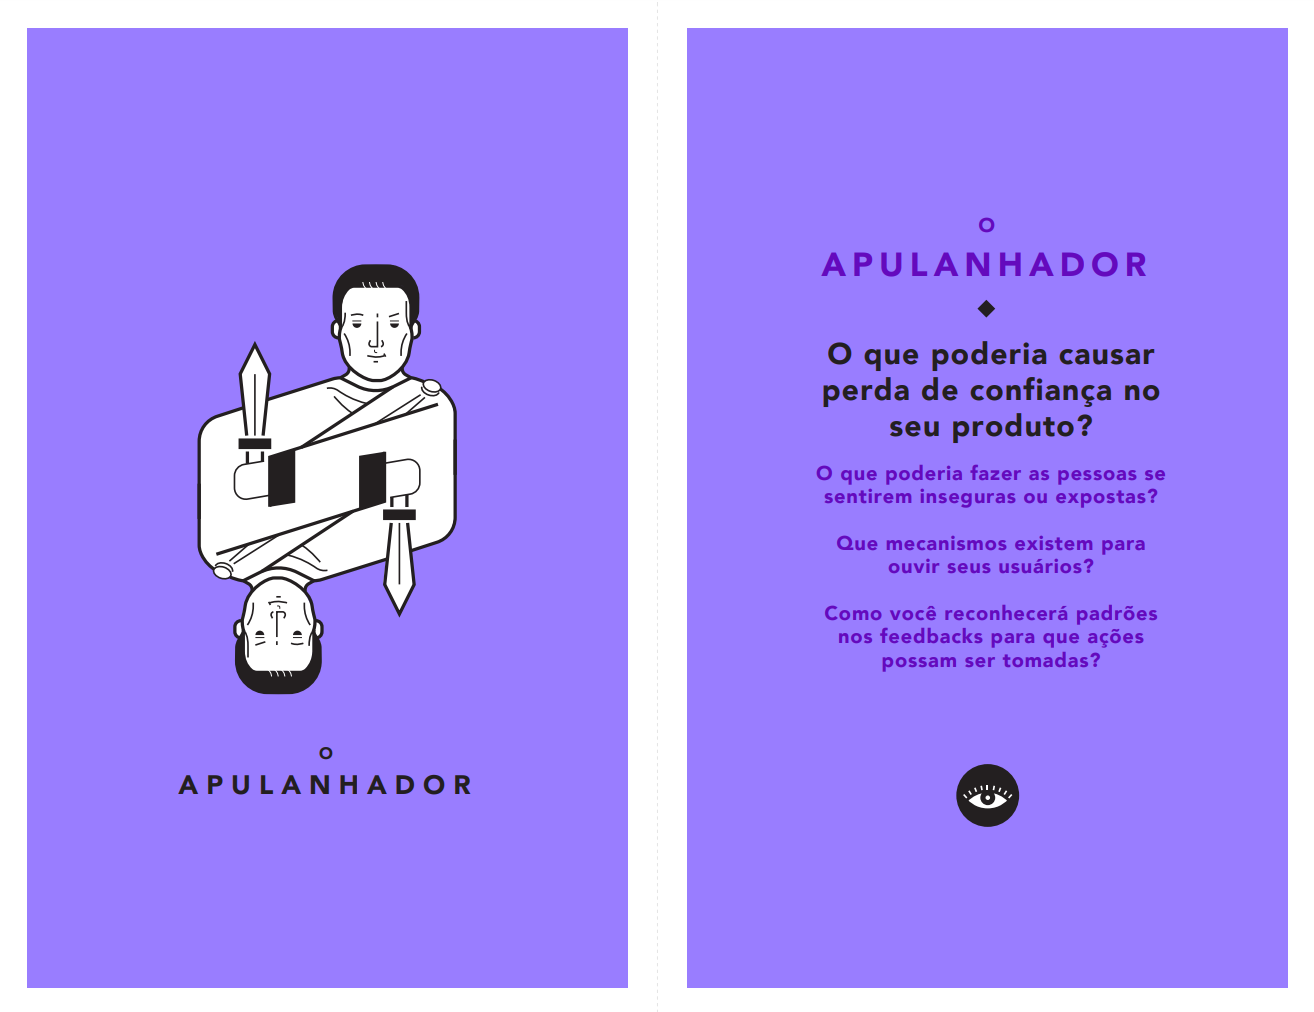
\includegraphics[width=\textwidth]{tarot-da-tecnologia}
	\legend{Fonte: Artefact}
\end{figure}

\subsubsection{Amarelinha / Board game}

O Amarelinha Game Board combina gamificação e análise de riscos em uma dinâmica interativa. O jogo segue uma trilha no estilo da amarelinha, com um participante de cada vez anunciando um risco identificado. Após o anúncio, todos os outros participantes categorizam o risco e calculam seu número de impacto, com base em sua probabilidade e severidade. Esse número representa a quantidade de casas que o participante avança no tabuleiro. O objetivo é alcançar o “céu” antes dos demais.

\begin{itemize}
  \item Vantagens: A dinâmica não apenas promove a identificação e categorização de riscos, mas também ensina os participantes a analisar impacto e probabilidade de maneira prática. É engajante e competitiva, o que pode aumentar a motivação.  
  \item Desvantagens: A competitividade pode desviar o foco de algumas equipes, especialmente se o objetivo for colaborativo. Além disso, a mecânica de calcular o número do risco pode ser desafiadora para equipes menos experientes, exigindo um facilitador.
\end{itemize}

Esta proposta tem viabilidade moderada. Exige preparação para definir categorias e criar o tabuleiro, mas pode ser adaptado com recursos básicos ou digitais.

\begin{figure}[H]
  \centering
  \caption{\label{amarelinha}Amarelinha caracol}
  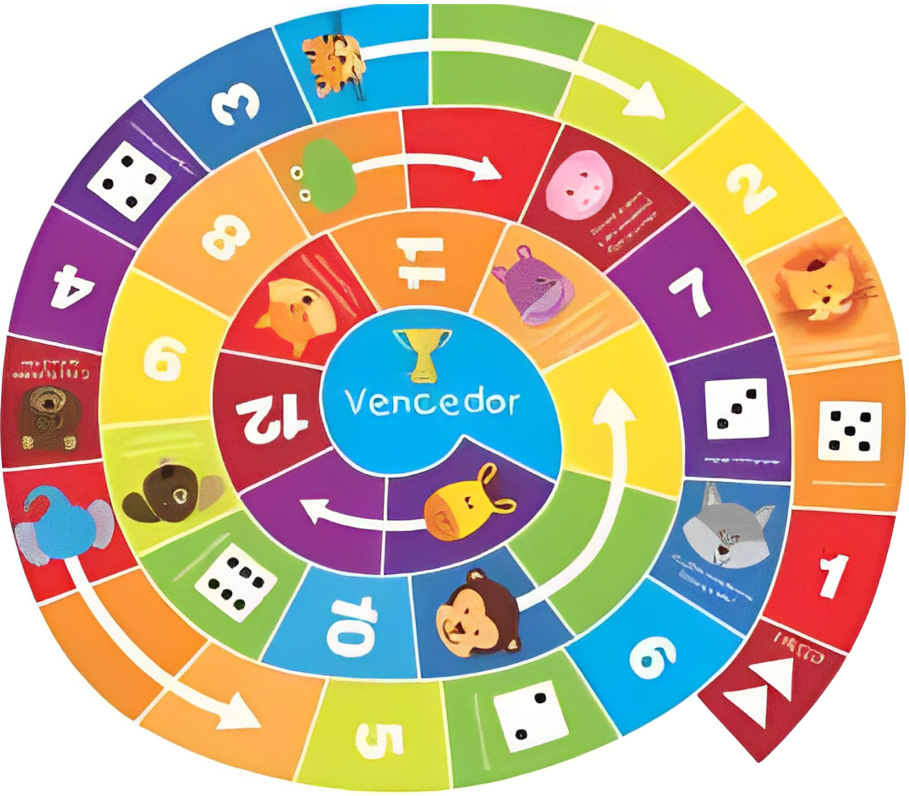
\includegraphics[width=0.8\textwidth]{amarelinha}
\end{figure}

\subsubsection{Poke risk}

O Poke Risk é inspirado no universo dos jogos de Pokémon, onde cada carta representa um risco que a equipe pode enfrentar. Antes do início do jogo, os participantes preenchem as cartas de riscos, atribuindo a elas parâmetros como probabilidade, impacto e cenário do risco. Essas cartas são usadas durante a dinâmica para promover a discussão, análise e priorização dos riscos identificados.

A partir do monte de cartas, todos os jogadores compram suas cartas, um por vez, até o monte acabar. Cada jogador estará representando determinados riscos durante a partida. Durante as rodadas, os participantes enfrentam "batalhas de riscos", onde anunciam o atributo com maiores chances de superar a carta do adversário. A carta ganhadora da batalha entra para um novo monte, que é o resultado dos riscos que devem ser priorizados para definição de estratégias de mitigação.

\begin{itemize}
  \item Vantagens: A abordagem lúdica torna a análise de riscos mais envolvente, especialmente para equipes que apreciam dinâmicas criativas.
  \item Desvantagens: Exige mais tempo de preparação e familiaridade dos participantes com o conceito dos parâmetros de risco. Sem um facilitador experiente, a dinâmica pode perder o foco ou se tornar menos produtiva.
\end{itemize}

Esta proposta tem viabilidade moderada. A preparação inicial das cartas exige tempo e alinhamento prévio, mas o processo de criação pode ser feito de forma colaborativa pela equipe, garantindo que as cartas sejam relevantes ao projeto.

\begin{figure}[H]
  \centering
	\caption{\label{super-trunfo}Super Trunfo Pokémon}
  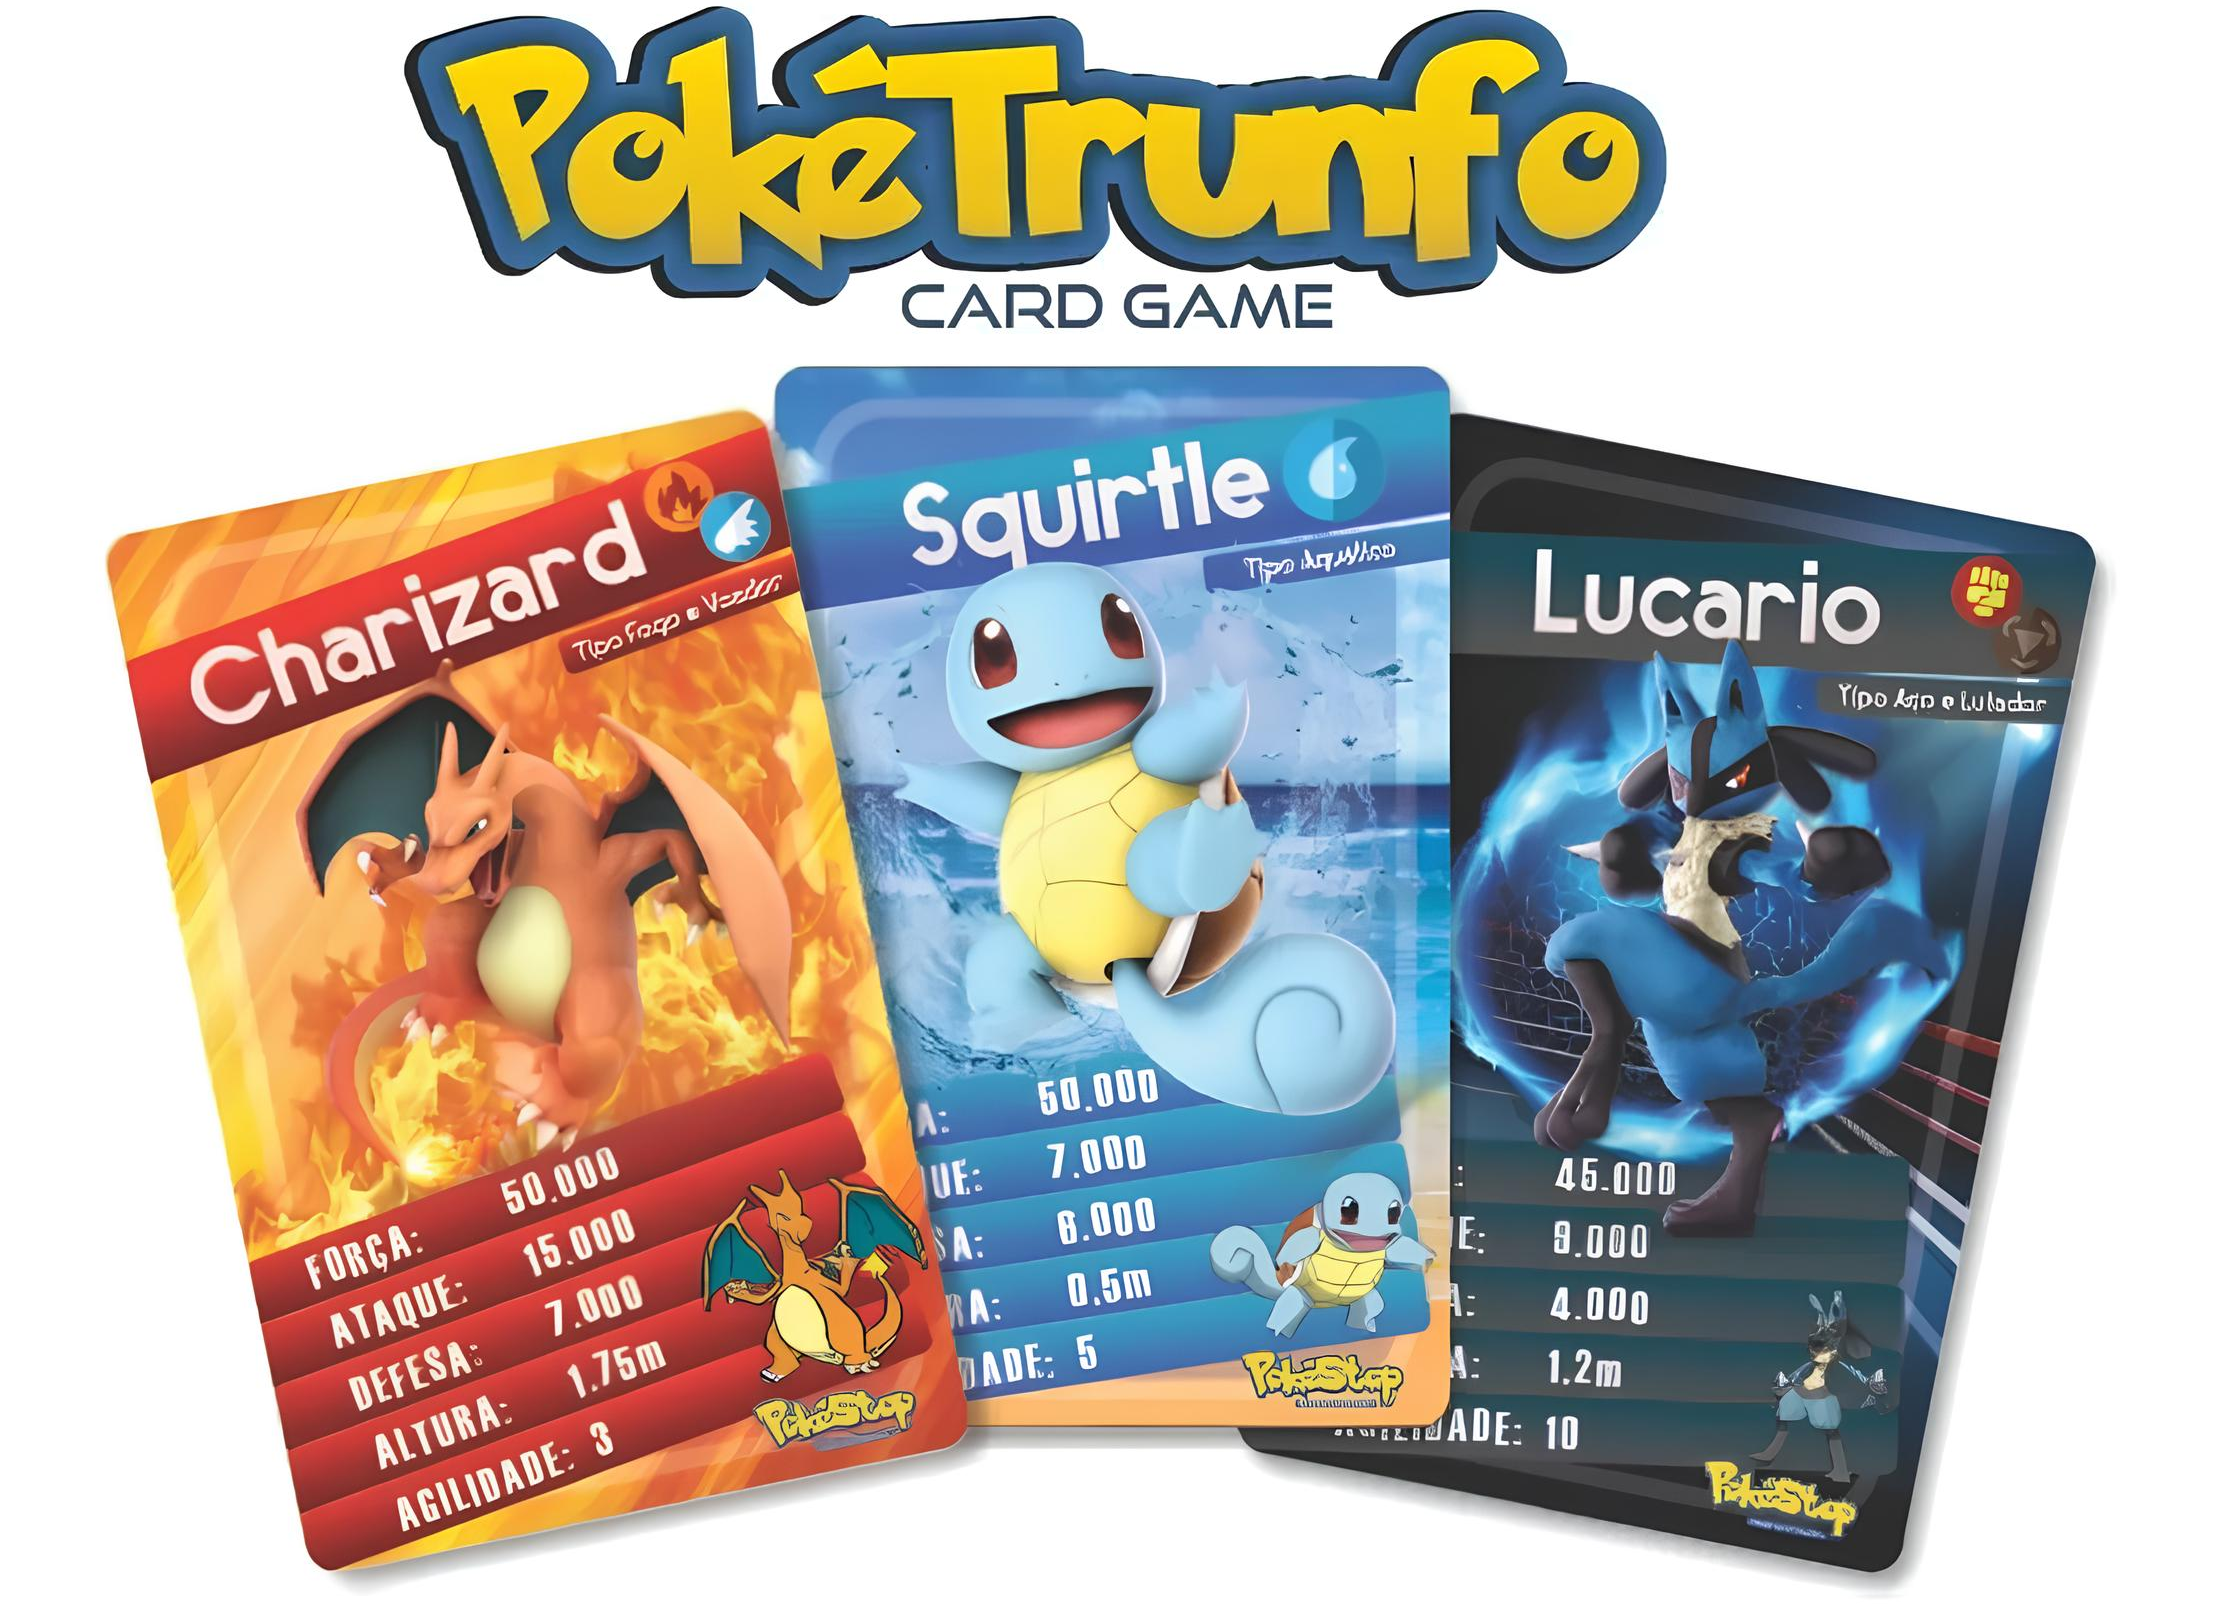
\includegraphics[width=0.8\textwidth]{super-trunfo}
\end{figure}


\section{Análise e design do jogo}

\section{Desenvolvimento da plataforma gamificada}

\section{Gerenciamento, monitoramento e medição}

%------------------------------------------------------------------------------%
%------------------------------------------------------------------------------%

\chapter{Dinâmica}

%------------------------------------------------------------------------------%
%------------------------------------------------------------------------------%

\chapter{Avaliação}

\section{Planejamento do estudo de caso}
\section{Realização do estudo de caso}
\section{Análise dos resultados do estudo de caso}

%------------------------------------------------------------------------------%
%------------------------------------------------------------------------------%

\chapter{Conclusão}

%------------------------------------------------------------------------------%


% Referências -----------------------------------------------------------------%

\postextual
\bibliography{tcc}

% Apêndices  -----------------------------------------------------------------%
\appendix

\chapter*{Apêndice A – Strings de busca adaptadas}
\addcontentsline{toc}{chapter}{Apêndice A – Strings de busca adaptadas}

\vspace{-2em}  % Ajusta o espaço negativo para reduzir a distância 

\begin{table}[h!]
  \centering
  \begin{tabular}{|l|p{12cm}|}
    \hline
    \textbf{Biblioteca digital} & \textbf{String adaptada} \\
    \hline
    ACM & (Title:(risk) OR Abstract:(risk)) AND (Title:(agile) OR Title:(scrum) OR Title:(xp) OR Title:(extreme programming) OR Title:(lean) OR Title:(kanban) OR Title:(scrumban) OR Title:(fdd) OR Title:(feature driven development) OR Title:(crystal) OR Title:(iterative development) OR Abstract:(agile) OR Abstract:(scrum) OR Abstract:(xp) OR Abstract:(extreme programming) OR Abstract:(lean) OR Abstract:(kanban) OR Abstract:(scrumban) OR Abstract:(fdd) OR Abstract:(feature driven development) OR Abstract:(crystal) OR Abstract:(iterative development)) AND (Title:(software) OR Abstract:(software)) \\
    \hline
    IEEExplore & "All Metadata":risk AND ("All Metadata":agile OR "All Metadata":scrum OR "All Metadata":xp OR "All Metadata":extreme programming OR "All Metadata":lean OR "All Metadata":kanban OR "All Metadata":scrumban OR "All Metadata":fdd OR "All Metadata":feature driven development OR "All Metadata":crystal OR "All Metadata":iterative development) AND "All Metadata":software \\
    \hline
    Scopus & (TITLE-ABS-KEY ( risk ) AND ( TITLE-ABS-KEY ( agile ) OR TITLE-ABS-KEY ( scrum ) OR TITLE-ABS-KEY ( xp ) OR TITLEABS-KEY ( extreme AND programming ) OR TITLE-ABS-KEY ( kanban ) OR TITLE-ABS-KEY ( scrumban ) OR TITLE-ABSKEY ( fdd ) OR TITLE-ABS-KEY ( feature AND driven AND development) OR TITLE-ABS-KEY ( crystal ) OR TITLE-ABS-KEY ( iterative AND development )) AND TITLE-ABS-KEY (software) AND ( LIMIT-TO ( SUBJAREA,"COMP") ) ) \\
    \hline
  \end{tabular}
\end{table}


\chapter*{Apêndice B – Estudos selecionados}
\addcontentsline{toc}{chapter}{Apêndice B – Estudos selecionados}

\vspace{-2em}  % Ajusta o espaço negativo para reduzir a distância

\begin{longtable}{|c|p{5.5cm}|p{7.5cm}|}
  \hline
  \textbf{Estudo} & \textbf{Título} & \textbf{Referência} \\
  \hline
  \endfirsthead
  \hline
  \multicolumn{3}{|c|}{\textit{Continua na próxima página}} \\
  \hline
  \endfoot
  \hline
  \multicolumn{3}{|c|}{\textit{Fim da tabela}} \\
  \hline
  \endlastfoot
  S1 & RM3: A Risk Management Framework for IT Project Success & Paulo Roberto Martins de Andrade and Samira Sadaoui. 2021. RM3: A Risk Management Framework For IT Project Success. In Proceedings of the 4th International Conference on Computer Science and Software Engineering (CSSE '21). Association for Computing Machinery, New York, NY, USA, 200–205. \\
  \hline
  S2 & A Risk Management Tool for Agile Software Development & Tavares, Breno \& Keil, Mark \& Sanches, Carlos \& Diniz de Souza, Adler \& Silva, Carlos. (2020). A Risk Management Tool for Agile Software Development. Journal of Computer Information Systems. 1. 1. 10.1080/08874417.2020.1839813. \\
  \hline
  S3 & A novel risk management model in the Scrum and extreme programming hybrid methodology & Afshari, Mahnaz \& Javdani Gandomani, Taghi. (2022). A novel risk management model in the Scrum and extreme programming hybrid methodology. International Journal of Electrical and Computer Engineering. 12. 2911-2921. 10.11591/ijece.v12i3.pp2911-2921. \\
  \hline
  S4 & Risk management framework in Agile software development methodology & Zahedi, Mohammad \& Kashanaki, Alireza \& Farahani, Elham. (2023). Risk management framework in Agile software development methodology. International Journal of Electrical and Computer Engineering (IJECE). 13. 4379. 10.11591/ijece.v13i4.pp4379-4387. \\
  \hline
  S5 & SERGE – Serious Game for the Education of Risk Management in Software Project Management & G. Annunziata, S. Lambiase, F. Palomba and F. Ferrucci, "SERGE - Serious Game for the Education of Risk Management in Software Project Management," 2024 IEEE/ACM 46th International Conference on Software Engineering: Software Engineering Education and Training (ICSE-SEET), Lisbon, Portugal, 2024, pp. 264-273, doi: 10.1145/3639474.3640085. \\
  \hline
  S6 & Do scaling agile frameworks address global software development risks? An empirical study & Beecham, Sarah \& Clear, Tony \& Lal, Ramesh \& Noll, John. (2021). Do scaling agile frameworks address global software development risks? An empirical study. Journal of Systems and Software. 171. 110823. 10.1016/j.jss.2020.110823. \\
  \hline
  S7 & User Story Risk Prioritization Model for Agile Software Development & P. Thanomwong and T. Senivongse, "User Story Risk Prioritization Model for Agile Software Development," 2022 International Conference on Data and Software Engineering (ICoDSE), Denpasar, Indonesia, 2022, pp. 161-166, doi: 10.1109/ICoDSE56892.2022.9972041. \\
  \hline
  S8 & Issues of Formalization of Risk Management Process in Software Design & BILOUSIVA, Liudmyla et al. Issues of formalization of risk management process in software design. In: IntelITSIS. 2023. p. 48-57. \\
  \hline
\end{longtable}

\chapter*{Apêndice C – Riscos categorizados}
\addcontentsline{toc}{chapter}{Apêndice C – Riscos categorizados}

\vspace{-2em}  % Ajusta o espaço negativo para reduzir a distância

%\renewcommand{\arraystretch}{1.2} 

\begin{longtable}{|>{\raggedright\arraybackslash}p{2.4cm}|p{4.5cm}|p{4.7cm}|l|}
  \hline
  \textbf{Classe} & \textbf{Elemento} & \textbf{Atributo} & \textbf{Estudo} \\
  \hline
  \endfirsthead
  \hline
  \multicolumn{4}{|c|}{\textit{Continua na próxima página}} \\
  \hline
  \endfoot
  \hline
  \multicolumn{4}{|c|}{\textit{Fim da tabela}} \\
  \hline
  \endlastfoot
  A. Product Engineering & 1. Requirements & a. Stability & S6, S7, S8 \\
  \cline{3-4}
  & & b. Completeness & S5, S7 \\
  \cline{3-4}
  & & c. Clarity & S5, S6, S7 \\
  \cline{3-4}
  & & d. Validity & S5, S6, S7 \\
  \cline{3-4}
  & & e. Feasibility & S5, S6, S7 \\
  \cline{3-4}
  & & g. Scale & S6 \\
  \cline{2-4}
  & 2. Design & b. Difficulty & S5 \\
  \cline{2-4}
  & 3. Code and Unit Test & a. Feasibility & S6 \\
  \cline{3-4}
  & & b. Testing & S8 \\
  \cline{2-4}
  & 5. Engineering Specialties & b. Reliability & S6 \\
  \hline
  B. Development Environment & 1. Development Process & c. Process Control & S6 \\
  \cline{3-4}
  & & d. Familiarity & S1 \\
  \cline{2-4}
  & 2. Development System & a. Capacity & S6 \\
  \cline{3-4}
  & & d. Familiarity & S6 \\
  \cline{2-4}
  & 3. Management Process & a. Planning & S1, S6 \\
  \cline{3-4}
  & & c. Management Experience & S6 \\
  \cline{3-4}
  & & d. Program Interfaces & S1 \\
  \cline{2-4}
  & 4. Management Methods & a. Monitoring & S6 \\
  \cline{3-4}
  & & b. Personnel Management & S6 \\
  \cline{2-4}
  & 5. Work Environment & a. Quality Attitude & S1 \\
  \cline{3-4}
  & & b. Cooperation & S5, S6 \\
  \cline{3-4}
  & & c. Communication & S1, S5, S6 \\
  \cline{3-4}
  & & d. Morale & S6 \\
  \cline{3-4}
  & & e. Reliability & S6 \\
  \hline
  C. Program Constraints & 1. Resources & a. Schedule & S1, S5, S6, S8 \\
  \cline{3-4}
  & & b. Staff & S1, S6, S8 \\
  \cline{3-4}
  & & c. Budget & S5, S6 \\
  \cline{2-4}
  & 2. Contract & c. Dependencies & S6 \\
  \cline{2-4}
  & 3. Program Interfaces & a. Customer & S6, S8 \\
  \cline{3-4}
  & & b. Associate Contractors & S1, S6 \\
  \cline{3-4}
  & & e. Corporate Management & S6 \\
  \cline{3-4}
  & & f. Vendors & S6 \\
  \cline{3-4}
  & & g. Politics & S6 \\
  \hline
\end{longtable}


%------------------------------------------------------------------------------%

\phantompart
\printindex

%------------------------------------------------------------------------------%

\end{document}